\documentclass[10pt, conference, compsocconf, letterpaper]{IEEEtranv17}

\pagestyle{plain}

\usepackage{algorithm}
%\usepackage{times}
\usepackage{amsmath}
\usepackage{amsthm}
\usepackage{graphicx}
\usepackage{color}
\usepackage{amssymb}
\usepackage[noend]{distribalgo}
\usepackage[draft]{fixme}
\usepackage{soul}
% natbib and cite added by me, not part of the ieeetran template!
%\usepackage[numbers]{natbib}
%\usepackage{cite}

\newcommand{\ex}{$\mathcal{E}$}
\newcommand{\pp}{$\mathcal{P}$}
\newcommand{\ppm}{\mathcal{P}}
\newcommand{\cc}{$\mathcal{C}$}
\newcommand{\ccm}{\mathcal{C}}
\newcommand{\vv}{$\mathcal{V}$}
\newcommand{\vvm}{\mathcal{V}}
\newcommand{\rr}{$\mathcal{R}$}
\newcommand{\rrm}{\mathcal{R}}
\newcommand{\sst}{$\mathcal{S}$}
\newcommand{\ssm}{\mathcal{S}}
\newcommand{\ts}{\text{\textit{ts}}}
\newcommand{\sendersTo}{\text{\textit{sendersTo}}}
\newcommand{\readv}{\text{\textit{read}}}
\newcommand{\writev}{\text{\textit{write}}}
\newcommand{\comp}{\text{\textit{computation}}}
\newcommand{\send}{\text{\textit{send}}}
\newcommand{\recv}{\text{\textit{receive}}}

\begin{document}

%\title{Scalable State-Machine Replication}
%
%
%\author{
%    \IEEEauthorblockN{Carlos Eduardo Bezerra\IEEEauthorrefmark{1}\IEEEauthorrefmark{3}, Fernando Pedone\IEEEauthorrefmark{1}, Robbert van Renesse\IEEEauthorrefmark{2}}
%    \IEEEauthorblockA  {
%       \IEEEauthorrefmark{1}University of Lugano,
%       \IEEEauthorrefmark{2}Cornell University,
%       \IEEEauthorrefmark{3}Universidade Federal do Rio Grande do Sul
%    }
%}

\title {Scalable State-Machine Replication\\[-3.0ex]}
\author {
    \IEEEauthorblockN {
        Carlos Eduardo Bezerra\IEEEauthorrefmark{1}\IEEEauthorrefmark{3},
        Fernando Pedone\IEEEauthorrefmark{1},
        Robbert van Renesse\IEEEauthorrefmark{2}
    }
    \IEEEauthorblockA {\IEEEauthorrefmark{1}University of Lugano, Switzerland}
    \IEEEauthorblockA {\IEEEauthorrefmark{2}Cornell University, USA}
    \IEEEauthorblockA {\IEEEauthorrefmark{3}Universidade Federal do Rio Grande do Sul, Brazil}
    \\[-3.0ex]
}

%\title{Scalable State-Machine Replication\\[3.0ex] 
%  {\normalfont\normalsize
%    Carlos Eduardo Bezerra\IEEEauthorrefmark{1}\IEEEauthorrefmark{3}, Fernando Pedone\IEEEauthorrefmark{1}, Robbert van Renesse\IEEEauthorrefmark{2}
%  }\\[-4.5ex]}
%
%\author{
%    \IEEEauthorblockA  {
%        \IEEEauthorrefmark{1}University of Lugano\\
%        Switzerland\\
%    }
%    \and
%    \IEEEauthorblockA  {
%        \IEEEauthorrefmark{2}Cornell University\\
%        United States of America
%    }
%    \and
%    \IEEEauthorblockA  {
%        \IEEEauthorrefmark{3}Universidade Federal do Rio Grande do Sul\\
%        Brazil
%    }
%}

\maketitle



\begin{abstract}
%Borrow from SSMR paper

%State machine replication (SMR) is a well-known technique to provide high availability and strong consistency (i.e., linearizability) to online services.
%In SMR, client commands are executed in the same order on all server replicas: after executing each client command, every replica will reach the same state. 
%%
%One problem is that the original SMR model lacks scalability, as every replica executes all commands.
%Because of that, adding replicas does not increase the maximum system throughput.
%%
%Scalable SMR (\ssmr) addresses this problem by partitioning the service state, allowing client commands to be executed only by some replicas, while still ensuring linearizability.
%By doing this, \ssmr\ scales linearly with the number of partitions for workloads where each command accesses a single partition.
%%
%However, \ssmr\ may quickly become saturated when executing multi-partition commands,
%as they require communication between partitions.
%Dynamic S-SMR (\dssmr) solves this problem by repartitioning the state dynamically, based on the workload.
%When a command needs variables from different partitions, those variables are first moved to the same partition.
%Then, the command is executed as a single-partition command.
%As a result, variables that are usually accessed together will tend to stay in the same partition, significantly improving scalability.
%We evaluate the performance of \dssmr\ with a scalable social network application.

State machine replication (SMR) is a well-known technique that guarantees strong consistency (i.e., linearizability) to online services.
In SMR, client commands are executed in the same order on all server replicas: after executing each command, every replica reaches the same state.
However, SMR lacks scalability: every replica executes all commands, so adding servers does not increase the maximum throughput.
Scalable SMR (\ssmr) addresses this problem by partitioning the service state, allowing commands to execute only in some replicas, providing scalability while still ensuring linearizability.
One problem is that ssmr quickly saturates when executing multi-partition commands,
as partitions must communicate.
\dssmrshort\ (\dssmr) solves this issue by repartitioning the state dynamically, based on the workload.
Variables that are usually accessed together are moved to the same partition, which significantly improves scalability.
We evaluate the performance of \dssmr\ with a scalable social network application.

\end{abstract}

%!TEX root =  main.tex
\section{Introduction}

State machine replication (SMR) is a well-established technique to develop highly available services (e.g., \cite{Shvachko:2003,Ghemawat:2003,Burrows:2006,MacCormick:2004}).
In essence, the idea is that replicas deterministically execute the same sequence of client commands in the same order and in doing so traverse the same sequence of states and produce the same results.
State machine replication provides configurable fault tolerance in the sense that the system can be set to tolerate any number of faulty replicas.
%Increasing the number of replicas, however, will not scale performance since each replica must execute every command.
Unfortunately, increasing the number of replicas will not scale performance since each replica must execute every command.

%For many online services, caping performance is a serious drawback.
Conceptually, scalable performance can be achieved with state partitioning (e.g., \cite{facebookTAO, sciascia2012sdur, Aguilera:2007}).
Ideally, if the service state can be divided such that commands access one partition only and are equally distributed among partitions, then system throughput (i.e., the number of commands that can be executed per time unit) will increase linearly with the number of partitions.
Although promising, exploiting partitioning in SMR is challenging.
First, most applications cannot be partitioned in such a way that commands always fall within a single partition.
Therefore, a partitioning scheme must cope with multi-partition commands.
Second, determining an efficient partitioning of the state is computationally expensive and requires an accurate characterization of the workload.

There are two general solutions to handle multi-partition commands.
One solution is to weaken the guarantees of commands that involve multiple partitions (e.g., \cite{facebookTAO}).
In the context of SMR, this would mean that single-partition commands are strongly consistent (i.e., linearizable) but multi-partition commands are not.
Another solution is to provide strong consistency guarantees for both single- and multi-partition commands, at the cost of a more complex execution path for commands that involve multiple partitions.
\ssmrlong\ (\ssmr)~\cite{bezerra2014ssmr} is a solution in this category.
\ssmr\ partitions the service state and replicates each partition.
It relies on an atomic multicast primitive to consistently order commands within and across partitions. 
Single-partition commands are multicast to their concerned partition and executed just like in classical SMR.
Multi-partition commands are multicast to all involved partitions; to prevent command interleaves that violate strong consistency, \ssmr\ implements execution atomicity.
With execution atomicity, partitions coordinate during the execution of multi-partition commands.
Unsurprisingly, multi-partition commands are more expensive than single-partition commands, and thus, the performance of \ssmr\ is particularly sensitive to the way the service state is partitioned.

Determining a partitioning of the state that avoids load imbalances and favors single-partition commands normally requires a good understanding about the workload. 
Even if enough information is available, finding a good partitioning is a complex optimization problem~\cite{curino2010sch,taft2014est}.
Moreover, many online applications experience variations in demand. 
These happen for a number of reasons. 
In social networks, some users may experience a surge increase in their number of followers (e.g., new ``celebrities");
workload demand may shift along the hours of the day and the days of the week; and unexpected (e.g., a video that goes viral) or planned events (e.g., a new company starts trading in the stock exchange) may lead to exceptional periods when requests increase significantly higher than in normal periods.
\ssmr\ assumes a static workload partitioning.
Any state reorganization requires system shutdown and manual intervention.

Given these issues, it is crucial that highly available partitioned systems be able to dynamically adapt to the workload.
In this paper, we present \dssmrlong\ (\dssmr), a technique that allows a partitioned SMR system to reconfigure its data placement on-the-fly.
\dssmr\ achieves dynamic data reconfiguration without sacrificing scalability or violating the properties of classical SMR.
These requirements introduce significant challenges.
Since state variables may change location, clients must find the current location of variables.
The scalability requirement rules out the use of a centralized oracle that clients can consult to find out the partitions a command must be multicast to.
Even if clients can determine the current location of the variables needed to execute a command, by the time the command is delivered at the involved partitions one or more variables may have changed their location.
Although the client can retry the command with the new locations, how to guarantee that the command will succeed in the second attempt?
In classical SMR, every command invoked by a non-faulty client always succeeds.
\dssmr\ should provide similar guarantees.

\dssmr\ was designed to exploit workload locality.
Our scheme benefits from simple manifestations of locality, such as commands that repeatedly access the same state variables, and more complex manifestations, such as structural locality in social network applications, where users with common interests have a higher probability of being interconnected in the social graph.
Focusing on locality allows us to adopt a simple but effective approach to state reconfiguration: whenever a command requires data from multiple partitions, the variables involved are moved to a single partition and the command is executed against this partition.
To reduce the chances of skewed load among partitions, the destination partition is chosen randomly.
Although \dssmr\ could use more sophisticated forms of partitioning, formulated as an optimization problem (e.g., \cite{curino2010sch,taft2014est}), our technique has the advantage that it does not need any prior information about the workload and is not computationally expensive.

To track object locations without compromising scalability, in addition to a centralized oracle that contains accurate information about the location of state variables, each client caches previous consults to the oracle.
As a result, the oracle is only contacted the first time a client accesses a variable or after a variable changes its partition.
Under the assumption of locality, we expect that most queries to the oracle will be accurately resolved by the client's cache.
To ensure that commands always succeed, despite concurrent relocations, after attempting to execute a command a few times unsuccessfully, \dssmr\ retries the command using \ssmr{}'s execution atomicity and involving all partitions. 
Doing so increases the cost to execute the command but guarantees that relocations will not interfere with the execution of the command.

We have fully implemented \dssmr\ as the \libname{} Java library, and we performed a number of experiments using \appname{}, a social network application built with \libname{}, with workloads exhibiting weak and strong locality.
We devised a mixed workload that estimates a real distribution of commands issued in a social network application.
Under such a workload, and with strong locality of access, \dssmr\ reached 74~kcps (thousands of commands per second), against less than 33~kcps achieved by \ssmr{}, improving by a factor of over 2.2.
With a weak-locality workload, \dssmr\ reached XX~kcps, against YY~kcps of \ssmr{}.

The paper makes the following contributions:
(1) It introduces \dssmr\ and discusses some performance optimizations, including the caching technique. 
(2) It details \libname{}, a Java library to simplify the design of services based on \dssmr{}.
(3) It describes \appname{} to demonstrate how \libname{} can be used to implement a scalable social network service.
(4) It presents a detailed experimental evaluation of \appname{}, deploying it with \ssmr\ and \dssmr{} in order to compare the performance of the two replication techniques.

The rest of the paper is structured as follows.
Section~\ref{sec:sysmodel} describes our system model.
Section~\ref{sec:background} reviews SMR and \ssmrshort{}.
Section~\ref{sec:dssmr} introduces \dssmr{}; we explain the technique in detail and argue about its correctness.
Section~\ref{sec:implementation} details the implementation of \libname\ and \appname{}.
Section~\ref{sec:experiments} reports on the results of our experiments with \dssmr{}.
Section~\ref{sec:rw} surveys related work and
Section~\ref{sec:conclusion} concludes the paper.







%!TEX root =  ssmr_ieee.tex

\section{Model and definitions}
\label{sec:model}

%In this section, we detail the system model and recall the notions of state-machine replication and linearizability, our correctness criterion.
%
%\subsection{Processes and communication}

We consider a distributed system consisting of an unbounded set of client processes $\ccm = \{c_1, c_2, ...\}$ and a bounded set of server processes $\ssm = \{s_1, ..., s_n\}$. 
Set $\ssm$ is divided into $P$ disjoint groups of servers, $\ssm_1, ..., \ssm_P$.
Processes are either \emph{correct}, if they never fail, or \emph{faulty}, otherwise. 
In either case, processes do not experience arbitrary behavior (i.e., no Byzantine failures).
Processes communicate by message passing, using either one-to-one or one-to-many communication, as defined next.
The system is asynchronous: there is no bound on message delay or on relative process speed.

One-to-one communication uses primitives $send(p,m)$ and $receive(m)$, where $m$ is a message and $p$ is the process $m$ is addressed to. 
If sender and receiver are correct, then every message sent is eventually received. 
%
One-to-many communication relies on atomic multicast, defined by the primitives \emph{multicast}$(\gamma, m)$ and \emph{deliver}$(m)$, where $\gamma$ is a set of server groups.
%where $g$ is the group message $m$ is addressed to, 
%
Let relation $\prec$ be defined such that $m \prec m'$ iff there is a server that delivers $m$ before $m'$.
Atomic multicast ensures that 
(i)~if a server delivers $m$, then all correct servers in $\gamma$ deliver $m$ \emph{(agreement)};
(ii)~if a correct process multicasts $m$ to groups in $\gamma$, then all correct servers in every group in $\gamma$ deliver $m$ \emph{(validity)}; and
(iii)~relation $\prec$ is acyclic \emph{(order)}.\footnote{Solving atomic multicast requires additional assumptions~\cite{CT96,FLP85}. In the following, we simply assume the existence of an atomic multicast oracle.}
%(ii)~if servers $s$ and $r$ deliver messages $m$ and $m'$, then they deliver them in the same order \emph{(order)}.
The order property implies that if $s$ and $r$ deliver messages $m$ and $m'$, then they deliver them in the same order. 
Atomic broadcast is a special case of atomic multicast in which there is a single group with all servers.



%!TEX root =  ssmr_ieee.tex

\section{Background and motivation}
%\section{State-machine replication}
\label{sec:smr}

State-machine replication is a fundamental approach to implementing a fault-tolerant service by replicating servers and coordinating the execution of client commands against server replicas~\cite{Lam78, Sch90}. 
The service is defined by a state machine, which consists of a set of \emph{state variables} $\vvm = \{v_1, ..., v_m\}$ 
%that encode the service's state 
and a set of \emph{commands} that may read and modify state variables, and produce a response for the command.
Each command is implemented by a deterministic program.
% whose execution is atomic with respect to other commands.
%The set of variables read by $C$ and the set of variables updated by $C$ are denoted, respectively, by $readset(C)$ and $writeset(C)$.
%The set of all variables read and updated by $C$ is denoted by $var(C)$. 
State-machine replication can be implemented with atomic broadcast: commands are atomically broadcast to all servers, and all correct servers deliver and execute the same sequence of commands.

We are interested in implementations of state-machine replication that ensure linearizability.
%
Linearizability is defined with respect to a sequential specification.
The \emph{sequential specification} of a service consists of a set of commands and a set of \emph{legal sequences of commands}, which define the behavior of the service when it is accessed sequentially.
In a legal sequence of commands, every response to the invocation of a command immediately follows its invocation, with no other invocation or response in between them.
For example, a sequence of operations for a read-write variable $v$ is legal if every read command returns the value of the most recent write command that precedes the read, if there is one, or the initial value otherwise.
An execution \ex\ is linearizable if there is some permutation of the commands executed in \ex\ that respects (i)~the service's sequential specification and (ii)~the real-time precedence of commands.
Command $C_1$ precedes command $C_2$ if the response of $C_1$ occurs before the invocation of $C_2$.

%The precise way in which the technique is implemented
%depends on the targeted consistency criterion, which in this paper we assume to be \emph{linearizability}. Once we prove that S-SMR provides such level of consistency, performance-optimized variations of S-SMR can be achieved later on by relaxing such consistency requirement. We can define linearizability intuitively: an execution in a replicated system is linearizable if the application program that uses such system gets the same behavior as with a single site, unreplicated system; hence, writing the application logic is no different to conventional programming~\cite{replication2010pedone}.

%To define linearizability more formally, we need the notion of \emph{sequential specification} for the variables, which determines whether a sequence of commands (and their matching responses) is legal, given a set of variables \mbox{$\vvm = \{v_1, ..., v_m\}$} stored in the servers. For example, the sequential specification for read-write variables is: given a sequence $\sigma$ of commands, the response given to any command $x$ that reads some variable $v$ must be coherent with the most recent command that writes $v$ and precedes $x$ in $\sigma$. Also, we need the notion of \emph{real-time precedence}, denoted by $<_{RT}$. We say that commands $x$ and $y$ are such that $x <_{RT} y$ if the response to command $x$ is received before command $y$ is issued, in real-time. Finally, execution \ex\ is linearizable if there is some permutation $\pi$ of the commands executed in \ex\, such that (i)~the sequential specification of every variable is respected in $\pi$ and (ii)~if $x <_{RT} y$, then $x$ precedes $y$ in $\pi$~\cite{Attiya04}.

%The execution in Fig.~\ref{fig:linvsnonlin} (top) is not linearizable because the reordering of commands that form a legal sequence (i.e., $C_1$, $C_3$, $C_2$) does not respect the real-time precedence of commands (i.e., it violates the real-time ordering of $C_2$ and $C_3$).
%%: we can see that $C_1 <_{RT} C_2 <_{RT} C_3$, but a permutation that respected such real-time precedence would not be legal. 
%In Fig.~\ref{fig:linvsnonlin} (bottom), however, there is no real-time precedence between $C_2$ and $C_3$, because $C_3$ was issued by client $b$ before client $a$ received the reply for $C_2$. For this reason, the execution is linearizable.
%
%\begin{figure}[ht]
%  \begin{center}
%    \begin{tabular}{c}
%      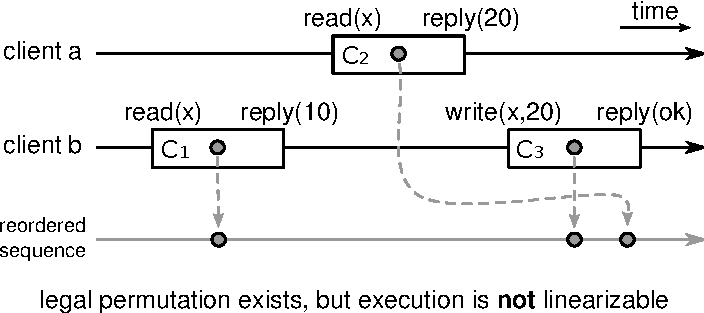
\includegraphics[width=0.9\columnwidth]{figures/nonlinearizable} \\
%      \\
%      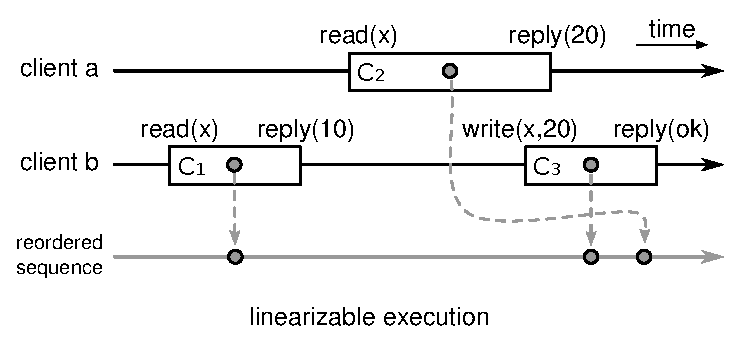
\includegraphics[width=0.9\columnwidth]{figures/linearizable} \\
%    \end{tabular}
%    \caption{Linearizable vs. non-linearizable executions.}
%    \label{fig:linvsnonlin}
%  \end{center}
%% \vspace{-4mm}
%\end{figure}


%State-machine replication implements linearizability by regulating how client commands are propagated to and executed by the replicas: 
%(i)~every nonfaulty replica must receive every command;  and
%(ii)~replicas must agree on the order of received and executed commands.
%Since each command is implemented by a deterministic program, each replica will produce the same state changes and response upon executing the same sequence of commands.
%State-machine replication can be implemented with atomic broadcast: commands are atomically broadcast to all servers, and all correct servers deliver and execute the same sequence of commands.
%%Since execution is deterministic, every server reaches the same state and produces the same response after executing a  command.

%\subsection{On the (lack of) scalability of SMR}

In classical state-machine replication, throughput does not scale with the number of replicas: each command must be ordered among replicas and executed and replied by every (non-faulty) replica.
Some simple optimizations to the traditional scheme can provide improved performance but not scalability.
For example, although update commands must be ordered and executed by every replica, only one replica can respond to the client, saving resources at the other replicas.
Commands that only read the state must be ordered with respect to other commands, but can be executed by a single replica, the replica that will respond to the client.

%A simple analysis shows that these schemes do not scale with the number of servers.
%Assume a replica needs $\delta_o$ time units to order a command, $\delta_e$ time units to execute the command, and $\delta_r$ time units to respond to the client---for simplicity, we consider $\delta_o$ to be constant with the number of servers.
%%~\cite{Marandi10}.
%In this model, traditional state-machine replication has throughput of $1/(\delta_o+\delta_e+\delta_r)$.
%The optimizations for update and read-only commands improve throughput to $N/(\delta_o+\delta_e+\delta_r/N)$ and $N/(\delta_o+(\delta_e+\delta_r)/N)$, respectively, where $N$ is the number of replicas.
%A scalable system would have throughput that grows proportionally with the number of servers.
%Figure~\ref{fig:scale} compares the behavior of traditional state-machine replication and the update and read-only optimizations with a truly scalable implementation. In the figure, we assume $\delta_o=\delta_e=\delta_r$; different values of $\delta$ would not change the asymptotic behavior of the techniques.
%
%
%\begin{figure}[ht]
%  \begin{center}
%      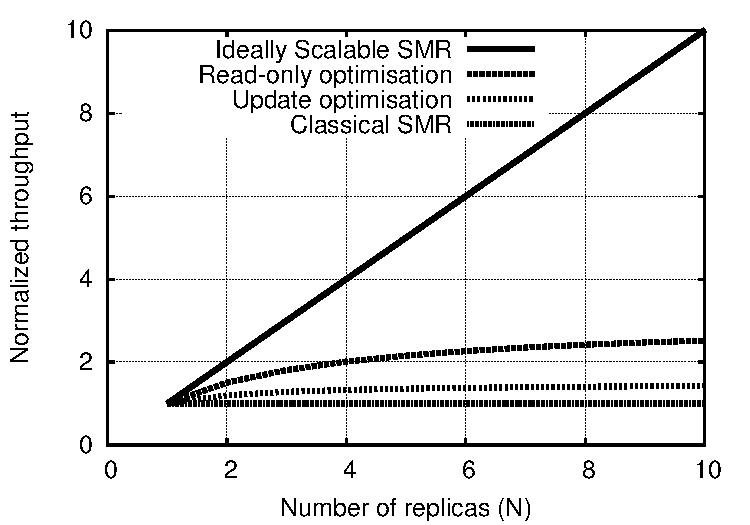
\includegraphics[width=0.9\columnwidth]{graphs/smr-scal/scale.pdf} 
%    \caption{Scalability of SMR implementations.}
%        \label{fig:scale}
%  \end{center}
%\end{figure}


%Such traditional implementations of SMR, however, has limited scalability. Adding servers to the system may not increase its throughput, and is likely, instead, to create a larger overhead on the group-communication component of the system, responsible for implementing atomic multicast. Note that servers can divide the execution of read-only commands (only one server has to execute, since no state is changed) and the sending of replies to write commands (although the state must change in all servers, one reply is enough). In the best case, i.e., in a workload dominated by read-only commands, this would approximate a linear increase of throughput, relatively to the number of servers. However, the group communication component of the system would have to increase its capacity as well, in order to avoid becoming a bottleneck, but its cost, in number of internal messages, would grow linearly (at least) to the number of processes in such component,\footnote{To the best of our knowledge, Ring-Paxos~\cite{Marandi10} requires the lowest number of messages for a consensus algorithm, which is $O(a)$, where $a$ is the number of acceptors.} eventually weighing out the linear (at best) throughput gain. In any case, even with a read-only workload, every server would have to deliver every single command, which alone would prevent the system from scaling.

This is a fundamental limitation: while some optimizations may increase throughput by adding servers, the improvements are limited since fundamentally, the technique does not scale.
In the next section, we describe an extension to SMR that under certain workloads allows performance to grow proportionally to the number of replicas.


%State-machine replication can be implemented with atomic multicast: if all servers belong to the same group and all commands are atomically multicast to such group, then all correct servers deliver and execute the same sequence of commands, i.e., they execute the commands in the same order. Moreover, if all servers have each a full copy of the application state, they all start at the same initial state, and command execution is deterministic, then every server reaches the same state after executing a given command and, thus, no two servers give different responses to the same command.



%\clearpage

%!TEX root =  ssmr_ieee.tex
\section{Scalable State-Machine Replication}
\label{sec:scalablesmr}

In this section, we introduce S-SMR, discuss performance optimizations, and argue about S-SMR's correctness.
%In this section, we introduce Scalable State-Machine Replication (S-SMR), describing its general idea (Section~\ref{sec:generalidea}) and detail its algorithm (Section~\ref{sec:detailalg}), discuss performance optimisations (Section~\ref{sec:optm}), and argue about S-SMR's correctness (Section~\ref{sec:correctness}).


%\subsection{Baseline approach}
\subsection{General idea}
\label{sec:generalidea}

S-SMR divides the application state $\vvm$ (i.e., state variables) into $P$ partitions $\ppm_1, ..., \ppm_P$, where for each $\ppm_i$, $\ppm_i \subseteq \vvm$. 
Moreover, we require each variable $v$ in $\vvm$ to be assigned to at least one partition and define $part(v)$ as the partitions that hold $v$. 
Each partition $\ppm_i$ is replicated by servers in group $\ssm_i$.
For brevity, we say that server $s$ belongs to $\ppm_i$ with the meaning that $s \in \ssm_i$, and say that client $c$ multicasts command $C$ to partition $\ppm_i$ meaning that $c$ multicasts $C$ to group $\ssm_i$.
% We also say that $\ppm_i$ does something meaning that servers in $\ssm_i$.
%We also often mention $\ppm_i$ meaning servers in $\ssm_i$.

To execute command $C$, the client multicasts $C$ to all partitions that hold a variable read or updated by $C$.
Consequently, the client must be able to determine the partitions accessed by $C$, denoted by $part(C)$.
Note that this assumption does not imply that the client must know all variables accessed by $C$, but it must know the partitions these variables belong to.
If the client cannot accurately estimate which partitions are accessed by $C$, it must determine a superset of these partitions, in the worst case assuming all partitions.
For performance, however, clients must strive to provide a close approximation to the command's actually accessed partitions. We assume the existence of an oracle that tells the client which partitions should receive each command.

Upon delivering command $C$, if server $s$ does not contain all variables read by $C$, $s$ must communicate with servers in other partitions to execute $C$. 
%
%can execute $C$ without and send the response to the client that issued $C$.
%%
%If $s$ stores only some of the variables accessed by $C$, $s$ must communicate with servers in other partitions to execute $C$. 
Essentially, $s$ must retrieve every variable $v$ read in $C$ from a server that stores $v$ (i.e., a server in a partition in $part(v)$).
Moreover, $s$ must retrieve a value of $v$ that is consistent with the order in which $C$ is executed, as we explain next.
Operations that do not involve reading a variable from a remote partition are executed locally.
%Server $s$ executes write operations that modify variables it stores and discards the other write operations.

%In more detail, assume that command $C$ is formed by a sequence of operations $op(C)$.
%Let $read(v)$ be an operation that reads the value of a state variable $v$ and $write(v, val)$ an operation that updates $v$ with value $val$.
%Any other operation may depend only on the state values read and the command's input.
%In the following, we assume that all read operations in a command precede the write operations.
%; we revisit this assumption in Section~\ref{sec:optm}.
%
%Server $s$ in partition $\ppm_i$ executes the $k$-th operation in $C$, $op(C)[k]$, as follows.

In more detail, let $op$ be an operation in the execution of command $C$.
We distinguish between three operation types: $read(v)$, an operation that reads the value of a state variable $v$, $write(v, val)$, an operation that updates $v$ with value $val$,
%and an operation that is neither a read nor a write.
and an operation that performs a deterministic computation.

Server $s$ in partition $\ppm_i$ executes $op$ as follows.

\begin{itemize}

\item[i)] \underline{$op$ is a $read(v)$ operation.} \\
If $\ppm_i \in part(v)$, then $s$ retrieves the value of $v$ and sends it to every partition $\ppm_j$ that delivers $C$ and does not hold $v$. If $\ppm_i \not\in part(v)$, then $s$ waits for $v$ to be received from a server in a partition in $part(v)$.

\item[ii)] \underline{$op$ is a $write(v,val)$ operation.} \\
If $\ppm_i \in part(v)$, $s$ updates the value of $v$ with $val$; if $\ppm_i \not\in part(v)$, $s$ executes $op$, creating a local copy of $v$, which will be up-to-date at least until the end of $C$'s execution.

\item[iii)] \underline{$op$ is a computation operation.}\\
In this case, $s$ executes $op$.

\end{itemize}

As we now show, the procedure above does not ensure linearizability.
Consider the execution depicted in Figure~\ref{fig:mcastnonlinssmr}~(a), where state variables $x$ and $y$ have initial value of $10$. 
Command $C_x$ reads the value of $x$, $C_y$ reads the value of $y$, and $C_{xy}$ sets $x$ and $y$ to value 20.
Consequently, $C_x$ is multicast to partition $\ppm_x$, $C_y$ is multicast to $\ppm_y$, and $C_{xy}$ is multicast to both $\ppm_x$ and $\ppm_y$. 
Servers in $\ppm_y$ deliver $C_y$ and then $C_{xy}$, while servers in $\ppm_x$ deliver $C_{xy}$ and then $C_x$, which is consistent with atomic order. 
In this execution, the only possible legal permutation for the commands is $C_y$, $C_{xy}$, and $C_x$, which violates the real-time precedence of the commands, since $C_x$ precedes $C_y$ in real-time.

%\begin{figure}[ht]
%  \begin{center}
%    \begin{tabular}{c}
%      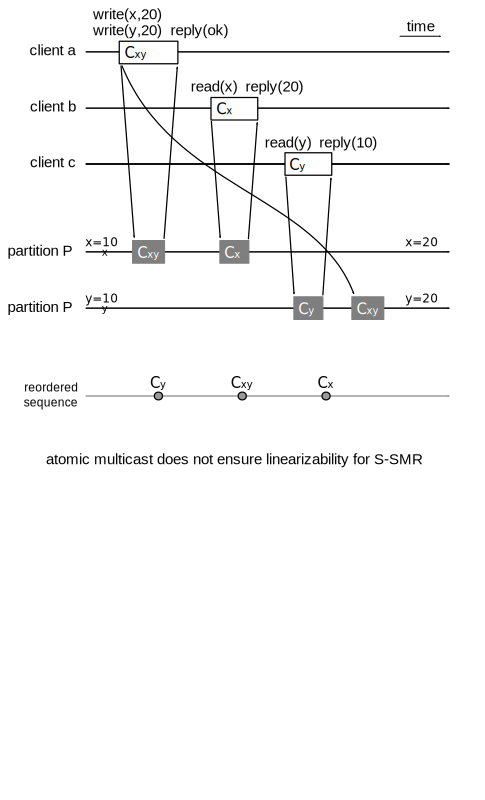
\includegraphics[width=0.9\columnwidth]{figures/mcastnonlinssmr} \\
%    \end{tabular}
%    \caption{Atomic multicast and S-SMR.}
%    \label{fig:mcastnonlinssmr}
%  \end{center}
%% \vspace{-4mm}
%\end{figure}
%
\begin{figure*}
\begin{minipage}[b]{1.0\linewidth} % A minipage that covers the whole width of the page
\centering
      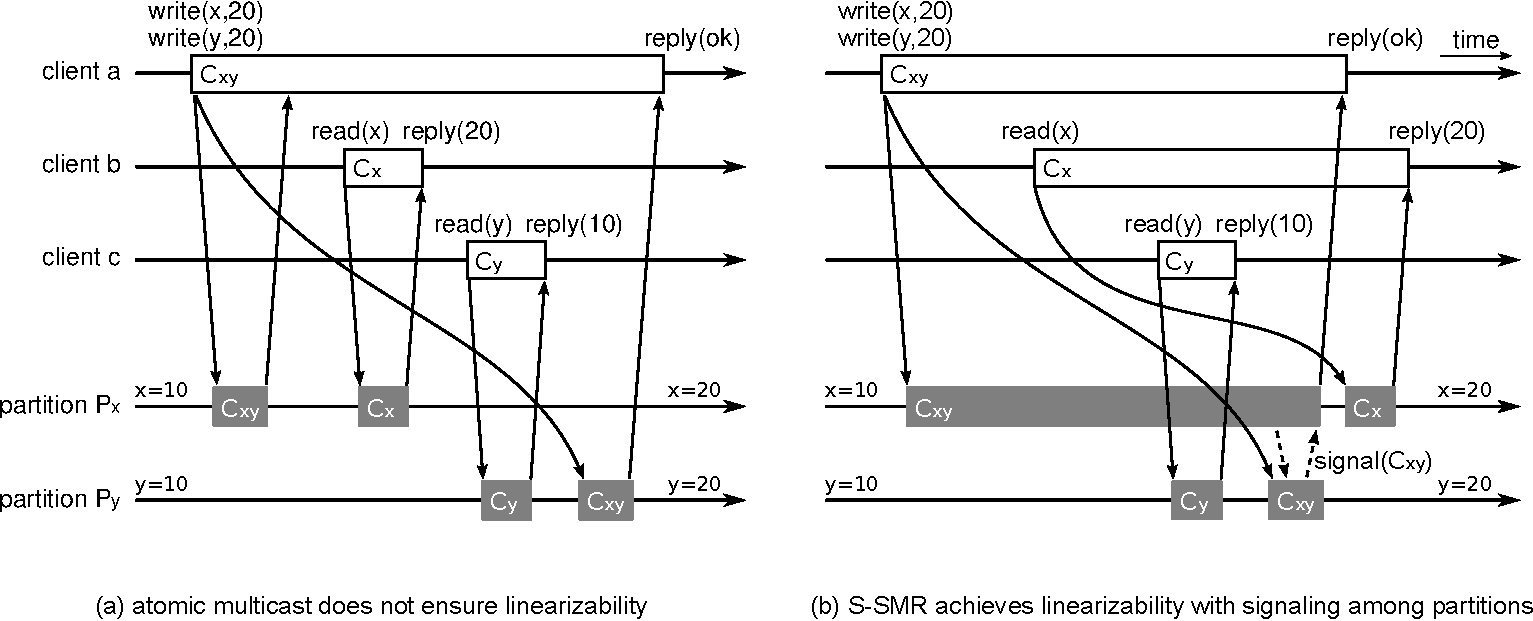
\includegraphics[width=0.85\linewidth]{figures/mcastssmr_nonlin_linsignal_v3}
\end{minipage}
%\begin{minipage}[b]{0.5\linewidth} % A minipage that covers half the page
%\centering
%      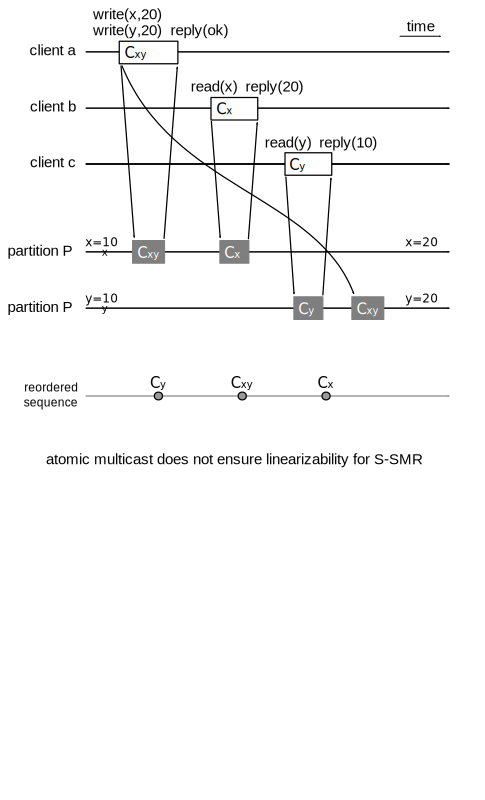
\includegraphics[width=0.9\columnwidth]{figures/mcastnonlinssmr}
%\end{minipage}
%\begin{minipage}[b]{0.5\linewidth}
%\centering
%      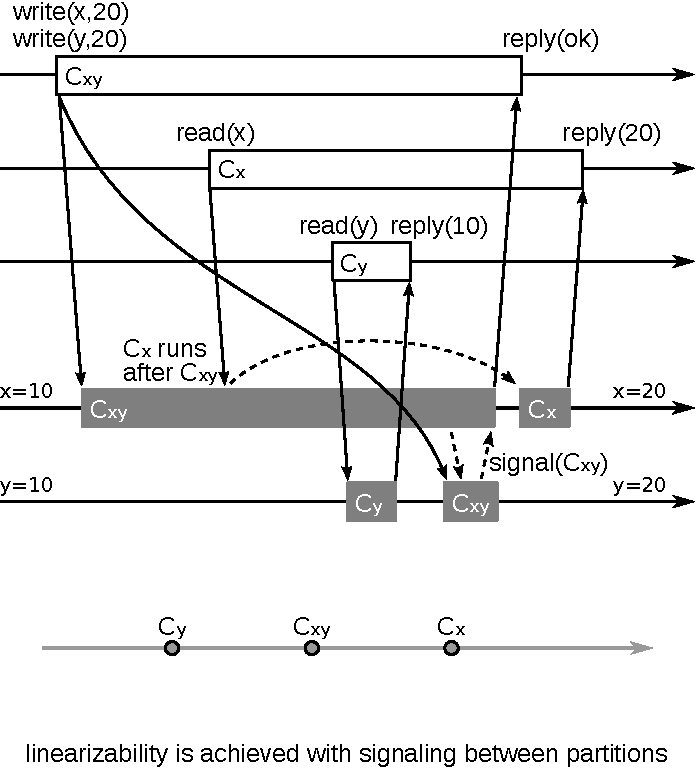
\includegraphics[width=0.9\columnwidth]{figures/mcastlinssmr_signal}
%\end{minipage}
\caption{Atomic multicast and S-SMR. (To simplify the figure, we show a single replica per partition.)}
\label{fig:mcastnonlinssmr}
\end{figure*}

Intuitively, the problem with the execution in Figure~\ref{fig:mcastnonlinssmr}~(a) is that commands $C_x$ and $C_y$ execute ``in between" the execution of $C_{xy}$ at partitions $\ppm_x$ and $\ppm_y$.
In S-SMR, we avoid such cases by ensuring that the execution of every command is atomic.
%
Command $C$ is \emph{execution atomic} if, for each server $s$ that executes $C$, there exists at least one server $r$ in every other partition in $part(C)$ such that the execution of $C$ at $s$ finishes after $r$ delivers $C$.
%
More precisely, let $delivery(C,s)$ and $end(C,s)$ be, respectively, the time when $s$ delivers command $C$ and the time when $s$ completes $C$'s execution.
Execution atomicity ensures that, for every server $s$ in partition \pp\ that executes $C$, there is a server $r$ in every $\ppm' \in part(C)$ such that $delivery(C,r) < end(C,s)$.
Intuitively, this condition guarantees that the execution of $C$ at $\ppm$ and $\ppm'$ overlap in time.

%Back in Fig.~\ref{fig:mcastnonlinssmr}, each black box represents the execution of a subcommand by servers in the partition: it starts when the first server in the partition begins executing the subcommand and ends when there is no more server executing the subcommand in that partition. We can see that $C_{xy}$ is not execution atomic: there is no time $t$ when some servers $s_x$ in $P_x$ and $s_y$ in $P_y$ are executing it. If it were the case, this example would be impossible to build, since $finish(C_y,s_y) < start(C_{xy}, s_y) < t < finish(C_{xy}, s_x) < start(C_x, s_x)$, which would contradict the fact that $C_x$ precedes $C_y$ in real-time.

Replicas can ensure execution atomicity by coordinating the execution of commands.
After delivering command $C$, servers in each partition send a $signal(C)$ message to servers in the other partitions in $part(C)$.
Before finishing the execution of $C$, each server must receive a $signal(C)$ message from at least one server in every other partition that executes $C$. 
%To minimize the waiting time to complete the execution of commands, servers may send such signal as soon as they deliver the command.
Moreover, if server $s$ in partition $\ppm$ receives the value of a variable from server $r$ in another partition $\ppm'$, as part of the execution of $C$, then $s$ does not need to receive a $signal(C)$ message from servers in $\ppm'$. This way, to tolerate $f$ failures, each partition requires $f+1$ servers; if all servers in a partition fail, service progress is not guaranteed.

Figure \ref{fig:mcastnonlinssmr}~(b) shows an execution of S-SMR. 
In the example, servers in $P_x$ wait for a signal from $P_y$, therefore delaying $C_{xy}$'s execution in $P_x$ and moving the execution of $C_x$ ahead in time. 
Note that the outcome of each command execution is the same as in case (a), but the executions of $C_x$, $C_y$ and $C_{xy}$, as seen by clients, now overlap in time with one another. 
Hence, there is no real-time precedence among them.

\subsection{Detailed algorithm}
\label{sec:detailalg}


\begin{algorithm}
\small
%\footnotesize
\begin{distribalgo}[1]
%\STATE \textbf{Algorithm 1:\\} Scalable State-Machine Replication (S-SMR)
\vspace{1mm}

\INDENT{\emph{Initialization:}}
    \STATE $\forall C \in \mathcal{K} : rcvd\_signals(C) \leftarrow \emptyset$
    \STATE $\forall C \in \mathcal{K} : rcvd\_variables(C) \leftarrow \emptyset$
\ENDINDENT

\vspace{1.5mm}
%\vspace{2.0mm}
\INDENT{\emph{Command $C$ is submitted by a client as follows:}}
    \STATE $dests \leftarrow oracle(C)$ \label{algline:oracle} 
%    \COMMENT{$oracle(C)$ returns a superset of $part(C)$}
	\STATE multicast$(dests, C)$ \label{algline:climcast}
	\STATE wait for response from one server
\ENDINDENT

\vspace{1.5mm}
%\vspace{2.0mm}
\INDENT{\emph{Command $C$ is executed by a server in partition \pp\ as follows:}}
	\INDENT{\textbf{upon} deliver$(C)$}
	    \STATE $others \leftarrow dests \setminus \{\ppm\}$ \label{algline:others}
	    \STATE multicast$(others, signal(C))$ \label{algline:mcastsignals}
		\FOR{each operation $op$ in $C$}
			\IF{$op$ is $read(v)$}
			    \IF{$v \in \ppm$}
			        \STATE multicast$(others, \{v,C.id\})$ \label{algline:multicastv}
			    \ELSE
			        \STATE \textbf{wait until} $v \in rcvd\_variables(C)$ \label{algline:waitvariable}
			        \STATE update $v$ with the value in $rcvd\_variables(C)$
			    \ENDIF
			\ENDIF
			\STATE execute $op$ \label{algline:executeopck}
		\ENDFOR
		\STATE \textbf{wait until} $rcvd\_signals(C) = others$ \label{algline:waitsignals}
		\STATE send reply to client \label{algline:sendreply}
	\ENDINDENT
	
	\vspace{2.0mm}
	\INDENT{\textbf{upon} deliver$(signal(C))$ from partition $\ppm'$}
	    \STATE $rcvd\_signals(C) \leftarrow rcvd\_signals(C) \cup \{\ppm'\}$
	\ENDINDENT

	\vspace{2.0mm}
	\INDENT{\textbf{upon} deliver$(\{v, C.id\})$}
	    \STATE $rcvd\_variables(C) \leftarrow rcvd\_variables(C) \cup \{v\}$
	\ENDINDENT
			
\ENDINDENT

\vspace{1.5mm}
%\vspace{2mm}

\textbf{Algorithm variables:}

\vspace{1mm}

$\mathcal{K}$: the set of all possible commands

\vspace{1mm}

$C.id$: unique identifier of command $C$

\vspace{1mm}

$oracle(C)$: function that returns a superset of $part(C)$

\vspace{1mm}

$dests$: set of partitions to which $C$ is multicast

\vspace{1mm}

$others$: set of partitions waiting for signals and variables from \pp; also, \pp\ waits for signals from all such partitions

\vspace{1mm}

$signal(C)$: a synchronization message that allows S-SMR to ensure $C$ to be execution atomic

\vspace{1mm}

$rcvd\_signals(C)$: a set containing all partitions that already signaled \pp\ regarding the execution of $C$

\vspace{1mm}

$rcvd\_variables(C)$: a set containing all variables that must be received from other partitions in order to execute $C$

\caption{Scalable State-Machine Replication (S-SMR)}
\label{alg:ssmr}
\end{distribalgo}
\end{algorithm}

In Algorithm \ref{alg:ssmr}, we show the basic operation of S-SMR. 
To submit a command $C$, the client queries an oracle to get set $dests$~(line \ref{algline:oracle}), which is a superset of $part(C)$ used by the client as destination set for $C$~(line \ref{algline:climcast}).

Upon delivering $C$, server $s$ in partition \pp\ multicasts $signal(C)$ to $others$, which is the set containing all other partitions involved in $C$ (lines \ref{algline:others} and \ref{algline:mcastsignals}). 
%The purpose of $signal(C)$ is to let servers in other partitions know that there is a server in \pp\ that started executing $C$. 
It might happen that $s$ receives signals concerning $C$ from other partitions even before $s$ started executing $C$. For this reason, $s$ must buffer signals and check if there are signals buffered already when starting the execution of $C$. For the sake of simplicity, Algorithm \ref{alg:ssmr} simply initializes such buffers as $\emptyset$ for all possible commands. In practice, buffers for $C$ are created when the first message concerning $C$ is delivered.

After multicasting signals, server $s$ proceeds to the execution of $C$, which is a sequence of operations that might read or write variables in \vv. The main concern is with operations that read variables, as they may determine the outcome of the command execution. All other operations can be executed locally at $s$. If the operation reads variable $v$ and $v$ belongs to \pp, $s$'s partition, then $s$ multicasts the value of $v$ to the other partitions that delivered $C$ (line \ref{algline:multicastv}). The command identifier $C.id$ is sent along with $v$ to make sure that the other partitions will use the appropriate value of $v$ during $C$'s execution. If $v$ belongs to some other partition $\ppm'$, $s$ waits until an up-to-date value of $v$ has been delivered (line \ref{algline:waitvariable}). Every other operation is executed with no interaction with other partitions (line \ref{algline:executeopck}).

After executing all operations of $C$, $s$ waits until a signal from every other partition has been received (line \ref{algline:waitsignals}) and, only then, sends the reply back to the client (line \ref{algline:sendreply}). This ensures that $C$ will be execution atomic.



\subsection{Performance optimizations}
\label{sec:optm}

Algorithm \ref{alg:ssmr} can be optimized in many ways. 
In this section, we briefly mention some of these optimizations and then detail caching.
\begin{itemize}
\item Server $s$ does not need to wait for the execution of command $C$ to reach a $read(v)$ operation to only then multicast $v$ to the other partitions in $part(C)$. If $s$ knows that $v$ will be read by $C$, $s$ can send $v$'s value to the other partitions as soon as $s$ starts executing $C$.
\item The exchange of objects between partitions serves the purpose of signaling. Therefore, if server $s$ sends variable $v$'s value to server $r$ in another partition, $r$ does not need to receive a signal message from $s$'s partition.
\item It is not necessary to exchange each variable more than once per command since any change during the execution of the command will be deterministic and thus any changes to the variable can be applied to the cached value.
\item Even though all replicas in all partitions in $part(C)$ execute $C$, a reply from a replica in a single partition suffices for the client to finish the command.
\end{itemize}

%Caching is a more elaborate optimization. 
Server $s$ in partition \pp\ can cache variables that belong to other partitions. 
There are different ways for $s$ to maintain cached variables; here we define two techniques: conservative caching and speculative caching. 
In both cases, the basic operation is the following: 
When $s$ executes a command that reads variable $x$ from some other partition $\ppm{}_x$, after retrieving the value of $x$ from a server in $\ppm{}_x$, $s$ stores $x$'s value in its cache and uses the cached value in future read operations.
If a command writes $x$, $s$ updates (or creates) $x$'s local value. 
Server $s$ will have a valid cache of $x$ until (i)~$s$ discards the entry due to memory constraints, or (ii)~some command not multicast to \pp\ changes the value of $x$. 
Since servers in $\ppm_x$ deliver all commands that access $x$, these servers know when any possible cached value of $x$ is stale.
How servers use cached entries distinguishes conservative from speculative caching.
%; what it does not know, however, is whether \pp\ has discarded $x$'s cache. 


Servers in $\ppm_x$ can determine which of its variables have a stale value cached in other partitions. This can be done by checking if there was any command that updated a variable $x$ in $\ppm_x$, where such command was not multicast to some other partition $\ppm$ that had a cache of $x$. Say servers in $\ppm_x$ deliver command $C$, which reads $x$, and say the last command that updated the value of $x$ was $C_w$. Since $x \in \ppm_x$, servers in $\ppm_x$ delivered $C_w$. One way for servers in $\ppm_x$ to determine which partitions need to update their cache of $x$ is by checking which destinations of $C$ did not receive $C_w$. This can be further optimized: even if servers in $\ppm$ did not deliver $C_w$, but delivered some other command $C_r$ that reads $x$ and $C_r$ was ordered by multicast after $C_w$, then $\ppm$ already received an up-to-date value of $x$ (sent by servers in $\ppm_x$ during the execution of $C_r$). If servers in $\ppm$ discarded the cache of $x$ (e.g., due to limited memory), they will have to send a request for its value.


\emph{Conservative caching}: Once $s$ has a cached value of $x$, before it executes a $read(x)$ operation, it waits for a cache-validation message from a server in $\ppm_x$. The cache validation message contains a set of pairs $(var, val)$, where $var$ is a state variable that belongs to $\ppm_x$ and whose cache in $\ppm$ needs to be validated. 
If servers in $\ppm_x$ determined that the cache is stale, $val$ contains the new value of $var$; otherwise, $\perp$, telling $s$ that its cached value is up to date.
If $s$ discarded its cached copy, it sends a request for $x$ to $\ppm_x$.
If it is possible to determine which variables are accessed by $C$ before $C$'s execution, all such messages can be sent upon delivery of the command, reducing waiting time; messages concerning variables that could not be determined a-priori are sent later, during the execution of $C$, as variables are determined.

\emph{Speculative caching}: It is possible to reduce execution time by speculatively assuming that cached values are up-to-date. 
Speculative caching requires servers to be able to rollback the execution of commands, in case the speculative assumption fails to hold. 
Many applications allow rolling back a command, such as databases, as long as no reply has been sent to the client for the command yet. 
The difference between speculative caching and conservative caching is that in the former servers that keep cached values do not wait for a cache-validation message before reading a cached entry; instead, a $read(x)$ operation returns the cached value immediately. 
If after reading some variable $x$ from the cache, during the execution of command $C$, server $s$ receives a message from a server in $\ppm_x$ that invalidates the cached value, $s$ rolls back the execution to some point before the $read(x)$ operation and resumes the command execution, now with the up-to-date value of $x$. 
%This may happen for every variable read by $C$, so $s$ might rollback the execution of $C$ several times until getting it right. 
%To ensure that a correct execution will be done eventually, 
Server $s$ can only reply to the client that issued $C$ after every variable read from the cache has been validated.

%Both caching algorithms depend on the following condition: each partition $\ppm_x$ keeps track of what was the last command $C$ executed by each partition $\ppm$, for each variable $x$ in $\ppm_x$, such that $C$ reads or writes $x$.\fixme{This part is too complicated.}
%Such values are kept by $\ppm_x$ in a table where each entry is $\langle \ppm, x, k \rangle$, where $k$ identifies the last command executed by $\ppm$ that accesses $x$. The initial value of $k$ is $0$ for every partition and every variable. Whenever a command $C$ that accesses $x$ is delivered by $\ppm_x$, it increments the command counter $k$ in $\langle \ppm, x, k \rangle$, for every partition $\ppm$ that delivers $C$. Upon delivery of any command $C'$ that also accesses $x$, $\ppm_x$ checks whether there is any partition $\ppm'$ that $C'$ was multicast to, where the cache of $x$ read by $C'$ will be stale, that is, entries $\langle \ppm_x, x, k \rangle$ and $\langle \ppm', x, k' \rangle$ are such that $k' < k$. Then, $P_x$ sends the cache-validation message(s) to $\ppm'$ accordingly.

\subsection{Correctness}
\label{sec:correctness}

In this proof, we denote the order given by atomic multicast with ``$\prec$''. Given any two messages $m_1$ and $m_2$, ``$m_1 \prec m_2$'' means that both messages are delivered by the same group and $m_1$ is delivered before $m_2$, or there is some message $m'$ such that $m_1 \prec m'$ and $m' \prec m_2$, which can be written as \mbox{$m_1 \prec m' \prec m_2$}.

We argue that, if every command in execution \ex\ of \mbox{S-SMR} is execution atomic, then \ex\ is linearizable. Suppose, by means of contradiction, that there exist two commands $x$ and $y$, where $x$ finishes before $y$ starts, but $y \prec x$ in the execution. There are two possibilities for this: (i) $x$ and $y$ access some variable in common $v$, or (ii) $x$ and $y$ access no variable in common.

In case (i), at least one partition $P_v$ (which contains $v$) delivers both $x$ and $y$. As $x$ finishes before $y$ starts, then $P_v$ delivers $x$, then $y$. From the properties of atomic multicast, and since each partition is mapped to a multicast group, no partition delivers $y$, then $x$. Moreover, atomic multicast ensures acyclic order, so there are no commands $z_1, ..., z_n$ such that their atomic order is $y \prec z_1 \prec \cdots \prec z_n \prec x$. So, we reached a contradiction in this case.

In case (ii), if there were no other command in \ex, then the execution of $x$ and $y$ could be done in any order, which would contradict the supposition that $y \prec x$. Therefore, there are commands $z_0, ..., z_n$ such that their atomic order is $y \prec z_0 \prec \cdots \prec z_n \prec x$. As $y \prec z_0$, then some partition $P_y$ delivers $y$, then $z_0$. Also, since $z_0 \prec z_1$, then some partition $P_1$ delivers $z_0$, then $z_1$, and so on: partition $P_i$ delivers $z_{i-1}$, then $z_i$, where $i \in \{1, ..., n\}$. Finally, partition $P_x$ delivers $z_n$, then $x$.

We now claim that for every $R_x \in P_x$, $R_x$ finishes executing $x$ only after some $R_0 \in P_0$ delivered $z_0$.
We prove our claim by induction.

Induction basis: As $z_n \prec x$, every $R_x \in Px$ executes command $x$ only after the execution of $z_n$ at $R_x$ finished. As $z_n$ is execution atomic, for every $R_x \in P_x$, there is a server $R_n \in P_n$ that delivered $z_n$ before $R_x$ finished executing $z_n$, which was before $R_x$ even started executing command $x$. Therefore, every $R_x \in P_x$ finishes executing $x$ only after some $R_n \in P_n$ delivered $z_n$.

Induction step: Assume that every $R_x \in P_x$ finishes executing $x$ only after some $R_i \in P_i$ delivered $z_i$. As $z_i$ is execution atomic, there is some $R_{i-1} \in P_{i-1}$ that delivered $z_i$ before $R_i$ finished executing $z_i$. As $z_{i-1} \prec z_i$ and $R_{i-1}$ delivers both, then $R_{i-1}$ delivers $z_{i-1}$ before executing $z_i$. Thus, $R_x \in P_x$ finishes executing $x$ only after some $R_{i-1}$ has delivered $z_{i-1}$, for every $R_x \in P_x$. This proves our claim.

Finally, for every $R_0 \in P_0$, there is a server $R_y \in P_y$ that delivers $z_0$ before $R_0$ finishes executing $z_0$. Since every $R_y$ delivers and executes $y$, then $z_0$, and from the claim above, for every $R_x \in P_x$, there is an $R_y \in P_y$ that delivers $y$ before $R_x$ finishes executing $x$. This contradicts the assumption that $x$ precedes $y$ in real-time, i.e., that the reply to $x$ is received before $y$ is invoked by a client.

% THE ALTERNATIVE BELOW ENDED UP EVEN MORE COMPLICATED!!!

% x = C_n
% y = C_1

%In this proof, we denote the order given by atomic multicast with ``$\prec$''. Given any two messages $m_1$ and $m_2$, ``$m_1 \prec m_2$'' means that both messages are delivered by the same group and $m_1$ is delivered before $m_2$, or there is some message $m'$ such that $m_1 \prec m'$ and $m' \prec m_2$, which can be written as \mbox{$m_1 \prec m' \prec m_2$}.
%
%We argue that, if every command in execution \ex\ of S-SMR is execution atomic, then \ex\ is linearizable. Suppose, by means of contradiction, that there exist two commands $C_1$ and $C_n$, where $C_1 \prec C_n$ in the execution, but $C_n$ finishes before $C_1$ starts. There are two possibilities for this: (i) $C_1$ and $C_n$ both access some variable in common $v$, or (ii) $C_1$ and $C_n$ access no variable in common.
%
%In case (i), at least one partition $P_v$ (which contains $v$) delivers both $C_1$ and $C_n$. As $C_n$ finishes before $C_1$ starts, then $P_v$ delivers $C_n$, then $C_1$. From the properties of atomic multicast, and since each partition is mapped to a multicast group, no partition delivers $C_1$, then $C_n$. Moreover, atomic multicast ensures acyclic order, so there are no commands $C_2, ..., C_{n-1}$ such that their atomic order is $C_1 \prec C_2 \prec \cdots \prec C_{n-1} \prec C_n$. So, we reached a contradiction in this case.
%
%In case (ii), if there were no other command in \ex, then there might be no partition that delivered both $C_1$ and $C_n$ and thus their execution could be done in any order, which would contradict the supposition that $C_1 \prec C_n$. Therefore, there are commands $C_2, ..., C_{n-1}$ such that their atomic order is $C_1 \prec C_2 \prec \cdots \prec C_{n-1} \prec C_n$. As $C_1 \prec C_2$, then some partition $P_1$ delivers $C_1$, then $C_2$. Also, since $C_2 \prec C_3$, then some partition $P_2$ delivers $C_2$, then $C_3$, and so on: partition $P_i$ delivers $C_i$, then $C_{i+1}$, where $i \in \{1, ..., n-1\}$.
%
%\textbf{Lemma}: For every server $R_{n-1} \in P_{n-1}$, $R_{n-1}$ finishes executing $C_n$ only after some server $R_1 \in P_1$ delivered $C_1$.
%
%We prove the proposition above by induction:
%
%Induction basis: As $C_{n-1} \prec C_n$, every $R_{n-1} \in P_{n-1}$ executes command $C_n$ only after the execution of $C_{n-1}$ at $R_{n-1}$ has finished. As $C_{n-1}$ is execution atomic, for every $R_{n-1} \in P_{n-1}$, there is a server $R_{n-2} \in P_{n-2}$ that delivered $C_{n-2}$ before $R_{n-1}$ finished executing $C_{n-1}$, which was before $R_{n-1}$ even started executing command $C_n$. Therefore, every $R_{n-1} \in P_{n-1}$ finishes executing $C_n$ only after some $R_{n-2} \in P_{n-2}$ started executing $C_{n-1}$.
%
%Induction step: Assume that every $R_x \in P_x$ finishes executing $x$ only after some $R_i \in P_i$ started executing $z_i$. As $z_i$ is execution atomic, there is some $R_{i-1} \in P_{i-1}$ that started execution $z_i$ before $R_i$ finished executing $z_i$. As $z_{i-1} \prec z_i$ and $R_{i-1}$ delivers both, then $R_{i-1}$ starts executing $z_{i-1}$ before executing $z_i$. Thus, $R_x \in P_x$ finishes executing $x$ only after some $R_{i-1}$ started executing $z_{i-1}$, for every $R_x \in P_x$. This proves Lemma 1.
%
%Finally, for every $R_0 \in P_0$, there is a server $R_y \in P_y$ that starts executing $z_0$ before $R_0$ finishes executing $z_0$. Since every $R_y$ delivers and executes $y$, then $z_0$, and from Lemma~1, for every $R_x \in P_x$, there is an $R_y \in P_y$ that starts executing $y$ before $R_x$ finishes executing $x$. This contradicts the assumption that $x$ precedes $y$ in real-time, i.e., that the reply to $x$ is received before $y$ is invoked by a client.
%


%!TEX root =  main.tex
\section{Implementation}
\label{sec:implementation}


Our  \dynastar prototype is written as a
Java \red{8?} library.
All code, including the experiment harness,
is publicly available with an open-source
license.\footnote{https://github.com/anonymous}
Application designers who use \dynastar
 to implement a replicated service must extend three key classes:
 \begin{itemize}
 \item[--] \emph{PRObject}: provides a common interface for (partially) replicated data items.
 \item[--] \emph{PartitionStateMachine}: encapsulates the logic of the server
   proxy. Note that the server logic is written without knowledge of the actual partitioning scheme. The \dynastar library
   handles all communication between partitions and the oracle transparently.
 \item[--] \emph{OracleStateMachine}: computes the mapping of objects to partitions.
Our default implementation uses the \red{METIS library} to provide an optimal partitioning based on the workload graph.
 \end{itemize}

 We note one important implementation detail.  The oracle is
 multi-threaded, and can service requests while computing a new
 partitioning concurrently. To ensure that all replicas start using
 the new partitioning consistently, the oracle identifies each
 partitioning with a unique id.  When an oracle replica finishes a
 repartitioning, it atomically multicasts the id of the new
 partitioning to all replicas of the oracle.  The first delivered id
 message defines the order of the new partitioning with respect to
 other oracle operations.





%% In this section, we describe \libname{}, a library that implements
%% both \ssmr{}, \dssmr{} and \dynastar{}.  We also present \appname{}, a
%% scalable social network application built with
%% \libname{}. \libname\ and \appname\ were both implemented in Java.

%% \subsection{\libname}

%% \libname{} implements functionalities of static and dynamic mapping,
%% and supports centralized and decentralized partitioning schemes.
%% There are three classes that the developer (i.e., application
%% designer) must extend to implement a replicated service with
%% \libname{}: PRObject, PartitionStateMachine, OracleStateMachine.

%% The \emph{PRObject class} represents any kind of data item that is
%% part of the service state. The state is partially replicated (i.e.,
%% objects are distributed among partitions). Therefore, when executing a
%% command, a replica might not have local access to some of the objects
%% involved in the execution of the command. The developer informs
%% \libname{} which object classes are partially replicated by extending
%% the PRObject class. Each object of such a class is stored locally or
%% remotely, but the application code is agnostic to the location of an
%% object. All calls to methods of such objects are intercepted by
%% \libname{}, transparently to the developer.

%% The \emph{PartitionStateMachine class} represents logic of the server
%% proxy. The application server class must extend the
%% PartitionStateMachine class. To execute commands, the developer must
%% provide an implementation for the method executeCommand(Command). The
%% code for such a method is agnostic to the existence of partitions. In
%% other words, developer programs for classical state machine
%% replication (i.e., full replication). \libname{} is responsible for
%% handling all communication between partitions and oracle
%% transparently. Objects that are involved in application's command will
%% be available to the partition at the time it is accessed by the
%% partitions. To start the server, method runStateMachine() is
%% called. Method createObject() also needs to be implemented, where the
%% developer defines how new state objects are loaded or created.


%% The \emph{OracleStateMachine class} defines the oracle, which is
%% deployed as a partition.  Because the oracle is in charge of moving
%% the PRObjects to the appropriate partitions, it requires a partitioner
%% that will provide for each object a desired location. A default
%% partitioner is implemented using METIS, a state-of-the-art graph
%% partitioner, but any algorithm that takes as input a graph and outputs
%% a mapping of objects to partitions is a valid partitioner.  The
%% workload graph is built by aggregating hints about the objects' access
%% patterns, and the mapping it returns indicates the ideal partition for
%% each object. Since the partitioner is executed in every oracle
%% replica, its output should be deterministic so all the replicas
%% transition to the same state after the partitioning.  The developer
%% can override the default algorithm to partition the graph and the
%% oracle is agnostic to its internal behavior.  At any time, the
%% application can request a repartitioning of the graph.


\subsection{\appname}
\label{sec:imp:\appname}

For the purposes of our evaluation, we have developed a Twitter-like
service named \appname{} using the \dynastar{} library.  With
\appname, users can follow, unfollow, post, or read other users'
tweets according to whom the user is following. Like Twitter, users
are constrained to posting 140-character messages.

Given that users in social networks spend most of the time reading
(i.e., performing getTimeline) \cite{facebookTAO}, we designed
\appname\ so that getTimeline are always a single-partition command.
Thus, when a user request a timeline, all posts are available in the
user's partition.  As a consequence, post, follow or unfollow commands
can lead to object moves.  Follow and unfollow commands can involve at
most two partitions, while posts can require object moves from one or
more partitions.


\subsection{Alternative Systems}

Throughout our evaluation, we compare \dynastar{} to two alternative
systems: S-SMR and DS-SMR. For performing our experiments, we used
the implementations of the two systems that are available in public
repositories. Since all three systems (S-SMR, DS-SMR, and Dynastar) provide
a common application-level interface, there was no additional work required
to port the \appname{} application. \rjs{We should add links to the repositories.}


%!TEX root =  ssmr_ieee.tex
\section{Performance Evaluation}
\label{sec:evaluation}

%In this section, we describe the environment in which we conducted our experiments, reason about our choice of benchmarks, and experimentally assess Scalable SMR by measuring the performance of the service we implemented on top of Eyrie.

In this section, we assess the performance of Volery with on-disk and in-memory deployments, and local and global commands.
%In this section, we assess the performance of Volery. 
%In Section \ref{sec:environment}, we describe the environment in which we conducted the experiments.
%%, as well as the parameters we used for the client and for the atomic multicast protocol.
%In Sections \ref{sec:disk} and \ref{sec:memory}, we present results for local commands, when Volery is configured with on-disk and in-memory storage, respectively.
%%In Section \ref{sec:memory}, we present the results when storage is done in memory only.
%In Section \ref{sec:global}, we evaluate Volery with global commands.

\subsection{Environment setup and configuration parameters}
\label{sec:environment}

We ran all our experiments on a cluster that had two types of nodes: (a) HP SE1102 nodes, equipped with two Intel Xeon L5420 processors running at 2.5 GHz and with 8 GB of main memory, and (b) Dell SC1435 nodes, equipped with two AMD Opteron 2212 processors running at 2.0 GHz and with 4 GB of main memory. The HP nodes were connected to an HP ProCurve Switch 2910al-48G gigabit network switch, and the Dell nodes were connected to an HP ProCurve 2900-48G gigabit network switch. Those switches were interconnected by a 20 Gbps link. 
%The round-trip latency between nodes connected to different switches was 0.13 ms on average.
All nodes ran CentOS Linux 6.3 with kernel 2.6.32 and had the Oracle Java SE Runtime Environment 7.
% with the \mbox{64-Bit} Server VM (build 24.0-b56).
Before each experiment, we synchronize the clocks of the nodes using NTP.
This is done to obtain accurate values in the measurements of the latency breakdown involving events in different servers.

In all our experiments with Volery and Zookeeper, clients submit commands asynchronously, that is, each client can keep submitting commands even if replies to previous commands have not been received yet, up to a certain number of outstanding commands. 
Trying to issue new commands when this limit is reached makes the client block until some reply is received. 
Replies are processed by callback handlers registered by clients when submitting commands asynchronously. 
We allowed every client to have up to 25 outstanding commands at any time. 
By submitting commands asynchronously, the load on the service can be increased without instantiating new client processes.
%Clients for both Volery and Chirper were implemented this way.
%Zookeeper offers such an asynchronous API, which we used in our experiments. 
Local commands consisted of calls to \verb#setData#, while global commands were invocations to \verb#create# and \verb#delete#. 
``Message size'' and ``command size'', in the next sections, refer to the size of the byte array passed to such commands.
% (except for deletions, which take only a path as parameter).


%We compared Volery with ZKsmr and with Zookeeper.

We compared Volery with the original Zookeeper and with ZKsmr, which is an implementation of the Zookeeper API using traditional state-machine replication. 
For the Zookeeper experiments, we used an ensemble of 3 servers. 
For the other approaches, we used Multi-Ring Paxos for atomic multicast, having 3 acceptors per ring: ZKsmr had 3 replicas that used one Paxos ring to handle all communication, while Volery had 3 replicas per partition, with one Paxos ring per partition, plus one extra ring for commands that accessed multiple partitions. 
Since Zookeeper runs the service and the broadcast protocol (i.e., Zab~\cite{ZAB2011}) in the same machines, each ZKsmr/Volery replica was colocated with a Paxos acceptor in the same node of the cluster. 
We had workloads with three different message sizes: 100, 1000 and 10000 bytes. 
Volery was run with 1, 2, 4 and 8 partitions. 
We conducted all experiments using disk for storage, then using memory (by means of a ramdisk). 
For on-disk experiments, we configured Multi-Ring Paxos with $\Delta$ \cite{MRPPROC2012} of 40 ms, batching timeout of 50 ms and batch size threshold of 250 kilobytes; for in-memory experiments, these parameters were 5 ms, 50 ms and 30 kilobytes, respectively.

%\begin{figure}[ht]
%  \begin{center}
%      \includegraphics[width=\columnwidth]{graphs/results/zk_disk/plot_tp_sizes} 
%    \caption{Normalized throughput versus command size.}
%        \label{fig:zktpdisk}
%  \end{center}
%\end{figure}

\subsection{Experiments using on-disk storage}
\label{sec:disk}

\begin{figure*}

\begin{minipage}[b]{0.5\linewidth} % A minipage that covers half the page
\centering
      \includegraphics[width=0.9\columnwidth]{{graphs/results/zk_disk/plot_tp_lat_multi_0.0readrate}.pdf}
\end{minipage}
\begin{minipage}[b]{0.5\linewidth}
\centering
      \includegraphics[width=0.9\columnwidth]{{graphs/results/zk_disk/timelines_all}.pdf}
\end{minipage}
\caption{Results for Zookeeper, ZKsmr and Volery (with 1, 2, 4 and 8 partitions) using disk. Throughput was normalized by that of Volery with a single partition (absolute values in kilocommands per second are shown). Latencies reported correspond to 75\% of the maximum throughput.}
\label{fig:zkdisk}
\end{figure*}



\begin{figure*}

\begin{minipage}[b]{0.3333\linewidth} % A minipage that covers half the page
\centering
      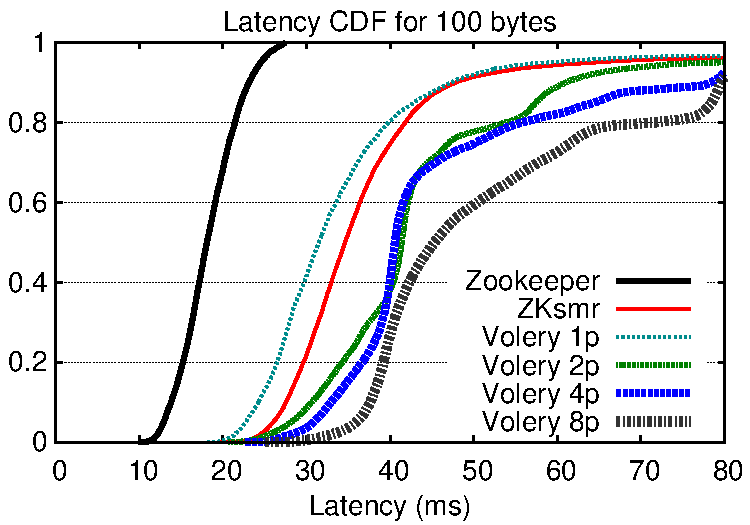
\includegraphics[width=0.9\columnwidth]{graphs/results/zk_disk/plot_latency_cdfs_100bytes}
\end{minipage}
\begin{minipage}[b]{0.3333\linewidth}
\centering
      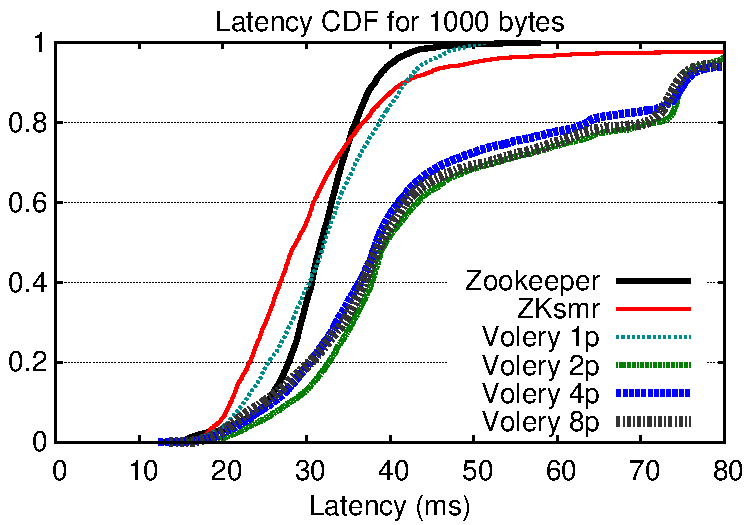
\includegraphics[width=0.9\columnwidth]{graphs/results/zk_disk/plot_latency_cdfs_1000bytes}
\end{minipage}
\begin{minipage}[b]{0.3333\linewidth}
\centering
      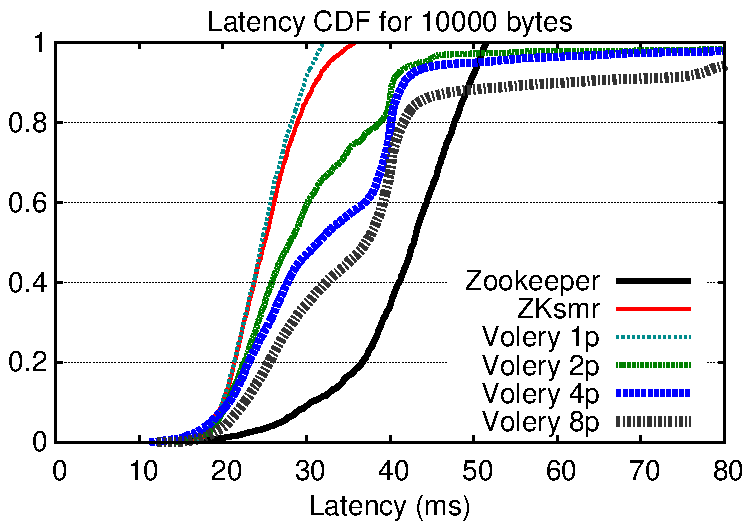
\includegraphics[width=0.9\columnwidth]{graphs/results/zk_disk/plot_latency_cdfs_10000bytes}
\end{minipage}
\caption{Cumulative distribution function (CDF) of latency for different command sizes (on-disk storage).}
\label{fig:zkdiskcdf}
\end{figure*}



In Figure \ref{fig:zkdisk}, we show results for local commands only.
%Each Paxos acceptor used BerkeleyDB for persistency, where each commit was synchronously written to disk. 
Each Paxos acceptor wrote its vote synchronously to disk before accepting each proposal. 
%Zookeeper was also configured to persist data to disk. 
Zookeeper also persisted data to disk. 
In Figure \ref{fig:zkdisk} (top left), we can see the maximum throughput for each replication scheme and message size, normalized by the throughput of Volery with a single partition. 
In all cases, the throughput of Volery scaled with the number of partitions and, for message sizes of 1000 and 10000 bytes, it scaled linearly (ideal case). 
%
%We can also see that, although Zookeeper had similar or higher throughput than Volery with one partition, having 4 partitions in Volery was enough to make it reach a higher throughput than Zookeeper, in all cases. 
%
For small messages (100 bytes), Zookeeper has similar performance to Volery with a single partition.
As messages increase in size, Zookeeper's throughput improves with respect to Volery: with 1000-byte messages, Zookeeper's throughput is similar to Volery's throughput with two partitions.
For large messages (10000 bytes), Zookeeper is outperformed by Volery with four partitions.
%
Comparing S-SMR with traditional SMR, we can see that for small messages (100 bytes), ZKsmr performed better than Volery with one partition. 
This is due to the additional complexity added by Eyrie in order to ensure linearizability when data is partitioned. 
Such difference in throughput is less significant with bigger commands (1000 and 10000 bytes).

We can also see in Figure \ref{fig:zkdisk} (bottom left), the latency values for the different implementations tested. 
Latency values correspond to 75\% of the maximum throughput.
Zookeeper has the lowest latency for 100- and 1000-byte command sizes. 
For 10000-byte commands, Volery had similar or lower latency than Zookeeper. 
Such lower latency of Volery with 10000-byte commands is due to a shorter time spent with batching: as message sizes increase, the size threshold of the batch (250 kilobytes for on-disk storage) is reached faster, resulting in lower latency. %Evidence for this phenomenon is given in Figure \ref{fig:zkdisk} (right).

Figure \ref{fig:zkdisk} (right) shows the latency breakdown of commands executed by Volery.
% down into its components, showing how much time is spent in each phase of the command's path between the client sending the command until the end of the command's execution. 
\emph{Batching} is the time elapsed from the moment the client sends command $C$ to the instant when $C$ is proposed by the ring coordinator as part of a batch. 
\emph{Multicasting} is the time between the propose is executed until the batch that contains $C$ is delivered by a server replica. 
\emph{Waiting} represents the time between the delivery and the moment when $C$ finally starts executing.
\emph{Executing} measures the delay between the start of the execution of command $C$ until the client receives $C$'s response.
We can see that more than half of the latency time is due to multicasting, which includes saving Multi-Ring Paxos instances synchronously to disk. 
There is also a significant amount of time spent with batching, done to reduce the number of disk operations and allow higher throughput: each Paxos proposal is saved to disk synchronously, so increasing the number of commands per proposal (i.e., per batch) reduces the number of times the disk is accessed.
%This allows performance to increase, but comes at the cost of increased latency.
This allows performance to improve, but increases latency.

%Having a more complex implementation, which took partitioning into account, made Volery have a higher average latency than ZKsmr and Zookeeper. As the message size increased, all approaches had higher latency, although there did not seem to exist a correlation of increased latencies as the number of partitions increased, in these experiments.

In Figure \ref{fig:zkdiskcdf}, we show the cumulative distribution functions (CDFs) of latency for all experiments where disk was used for storage. 
The results show that the latency distributions for ZKsmr and Volery with a single partition are similar, while latency had more variation for 2, 4 and 8 partitions. 
An important difference between deployments with a single and with multiple partitions is related to how Multi-Ring Paxos is used. In ZKsmr and in Volery with a single partition, there is only one Paxos ring, which orders all commands from all clients and delivers them to all replicas. 
When there are multiple partitions, each replica delivers messages from two rings: one ring that orders messages related to the replica's partition only, and another ring that orders messages addressed to more than one partition---each replica deterministically merges deliveries from multiple rings. 
As the time necessary to perform such deterministic merge is influenced by the level of synchrony of the rings, latency is expected to fluctuate more when merging is involved.

\subsection{Experiments using in-memory storage}
\label{sec:memory}

\begin{figure*}

\begin{minipage}[b]{0.5\linewidth} % A minipage that covers half the page
\centering
      \includegraphics[width=0.9\columnwidth]{{graphs/results/zk_mem/plot_tp_lat_multi_0.0readrate}.pdf}
\end{minipage}
\begin{minipage}[b]{0.5\linewidth}
\centering
      \includegraphics[width=0.9\columnwidth]{{graphs/results/zk_mem/timelines_all}.pdf}
\end{minipage}
\caption{Results for Zookeeper, ZKsmr and Volery (with 1, 2, 4 and 8 partitions) using memory. Throughput was normalized by that of Volery with a single partition (absolute values in kilocommands per second are shown). Latencies reported correspond to 75\% of the maximum throughput.}
\label{fig:zkmem}

\end{figure*}



\begin{figure*}

\begin{minipage}[b]{0.3333\linewidth} % A minipage that covers half the page
\centering
      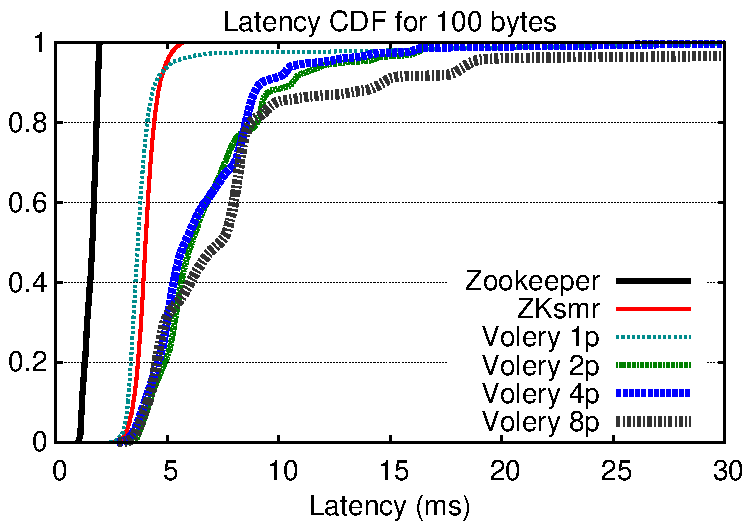
\includegraphics[width=0.9\columnwidth]{graphs/results/zk_mem/plot_latency_cdfs_100bytes}
\end{minipage}
\begin{minipage}[b]{0.3333\linewidth}
\centering
      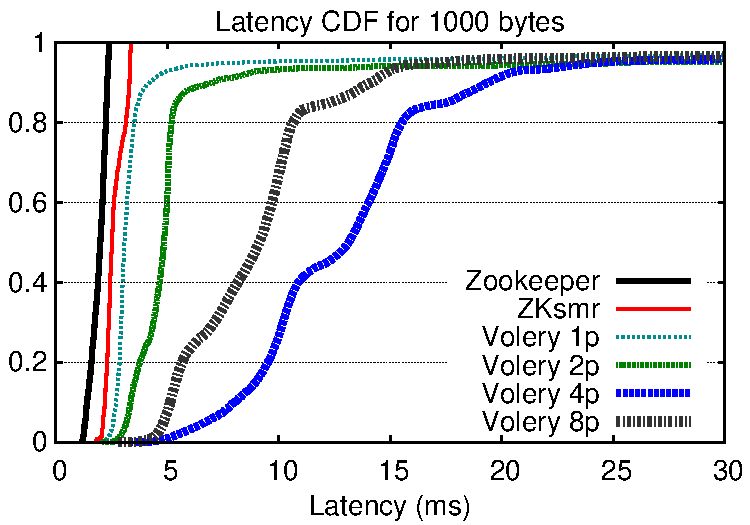
\includegraphics[width=0.9\columnwidth]{graphs/results/zk_mem/plot_latency_cdfs_1000bytes}
\end{minipage}
\begin{minipage}[b]{0.3333\linewidth}
\centering
      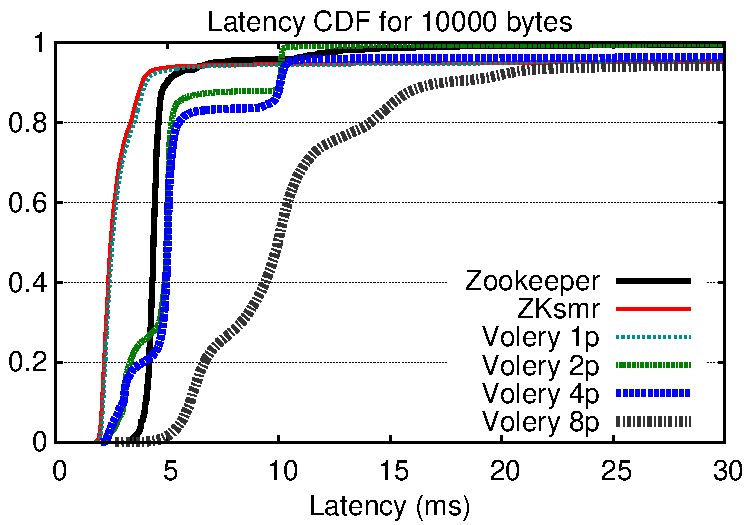
\includegraphics[width=0.9\columnwidth]{graphs/results/zk_mem/plot_latency_cdfs_10000bytes}
\end{minipage}
\caption{Cumulative distribution function (CDF) of latency for different command sizes (in-memory storage).}
\label{fig:zkmemcdf}
\end{figure*}

In Figure \ref{fig:zkmem}, we show the results for local commands when storing data in memory only. 
Volery's throughput scales with the number of partitions (Figure \ref{fig:zkmem} (top left)), specially for large messages, in which case the scalability is linear with the number of partitions (i.e., ideal case). 
We can also see that latency values for Volery and ZKsmr are less than half of what they are for on-disk storage (Figure \ref{fig:zkmem} (bottom left)), while Zookeeper's latency decreased by an order of magnitude. 
%The difference in latency is due to the atomic multicast library (URingPaxos) we use, while Zookeeper uses Zab, which is a greatly optimised atomic broadcast algorithm.
These results suggest that further improvements should be achievable in the in-memory Volery configuration with additional optimizations and finer tuning of the atomic multicast parameters.

Figure \ref{fig:zkmem} (right) shows the latency breakdown. 
Even though no data is saved to disk, multicasting is still responsible for most of the latency, followed by batching. 
Differently from the experiments described in Section \ref{sec:disk}, batching here had a size threshold of 30 kilobytes, which helps to explain why batching time is roughly the same for different message sizes. 
In these experiments, although there are no disk writes, batching is still used because it reduces the number of Paxos proposals and the number of messages sent through the network, which allows higher throughput. 
Figure~\ref{fig:zkmemcdf} shows the latency CDFs for the in-memory experiments, where we can see that Volery with multiple partitions (i.e., deployments where Multi-Ring Paxos uses multiple rings) tends to have more variation in latency.

\subsection{Experiments with global commands}
\label{sec:global}

In this section, we analyze how Volery performs when the workload includes commands that are multicast to all partitions (global commands). This is the least favorable (non-faulty) scenario for S-SMR, as having commands multicast to all partitions effectively reduces scalability: if all commands go to all partitions, adding more partitions will not increase throughput.

We ran experiments with different rates of global commands (i.e., create and delete operations): 0\%, 1\%, 5\% and 10\% of all commands. 
We chose such rates for two reasons: (i) it is obvious that high rates of global commands will prevent the system from scaling, plus (ii) it is common for large scale services to have a high rate of read requests (which are local commands in Volery). 
An example of such a service is Facebook's TAO~\cite{facebookTAO}, which handles requests to a social graph; it allows, for instance, pages to be generated based on the user's connections in the social network. 
In Facebook's TAO, 99.8\% of all requests are read-only~\cite{facebookTAO}. 
%With this kind of workload in mind, 10\% is a \emph{very} high rate of global commands.

\begin{figure*}

\begin{minipage}[b]{0.5\linewidth} % A minipage that covers half the page
\centering
      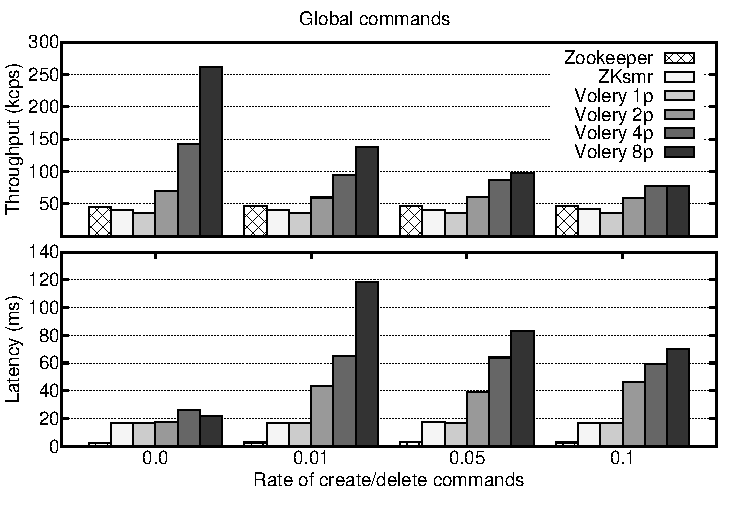
\includegraphics[width=0.9\columnwidth]{{graphs/results/zk_multipartition/plot_tp_lat_multi_global}.pdf}
\end{minipage}
\begin{minipage}[b]{0.5\linewidth}
\centering
      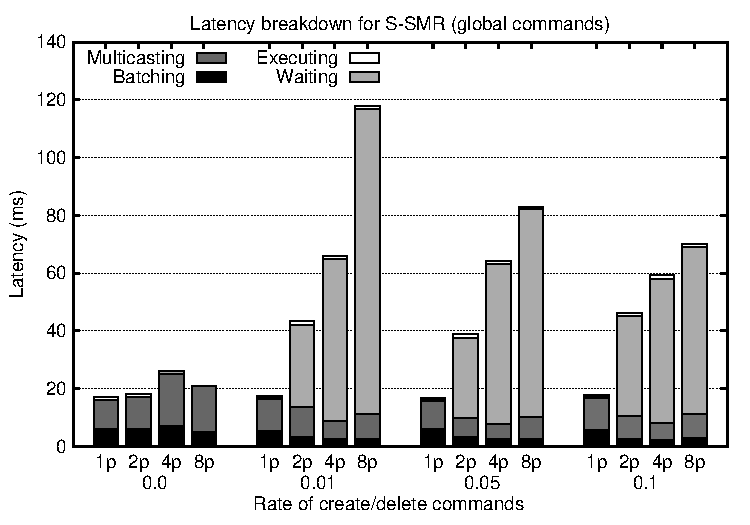
\includegraphics[width=0.9\columnwidth]{{graphs/results/zk_multipartition/timelines_global}.pdf}
\end{minipage}
\caption{Throughput and latency versus rate of create/delete commands (in-memory storage, 1000-bytes commands). Throughput is shown in units of a thousand commands per second (kcps). Latencies shown corresponds to 75\% of the maximum throughput.}
\label{fig:zkglobal}
\end{figure*}

\begin{figure*}

\begin{minipage}[b]{0.3333\linewidth} % A minipage that covers half the page
\centering
      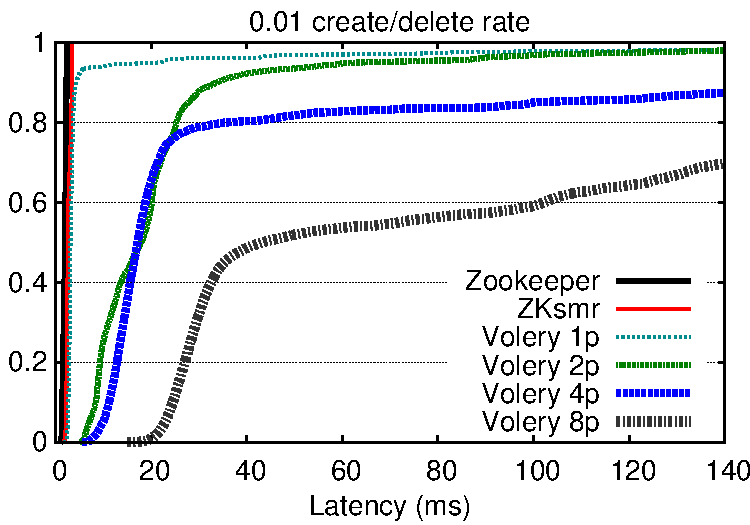
\includegraphics[width=0.9\columnwidth]{{graphs/results/zk_multipartition/plot_latency_cdfs_globalrate_0.01}.pdf}
\end{minipage}
\begin{minipage}[b]{0.3333\linewidth}
\centering
      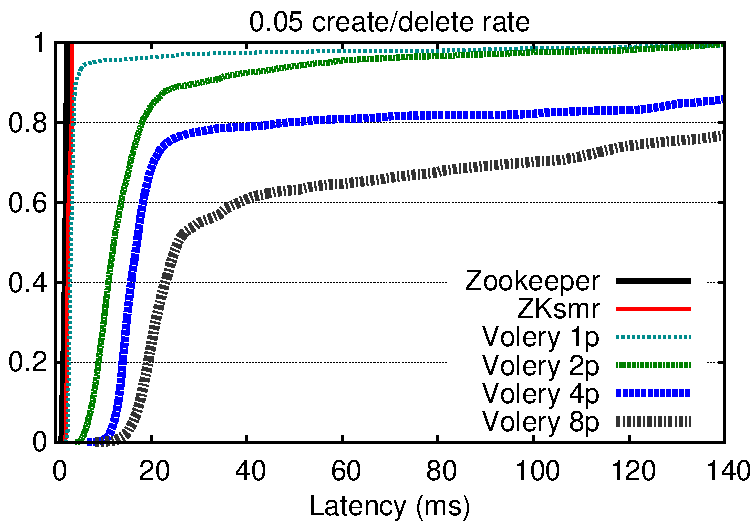
\includegraphics[width=0.9\columnwidth]{{graphs/results/zk_multipartition/plot_latency_cdfs_globalrate_0.05}.pdf}
\end{minipage}
\begin{minipage}[b]{0.3333\linewidth}
\centering
      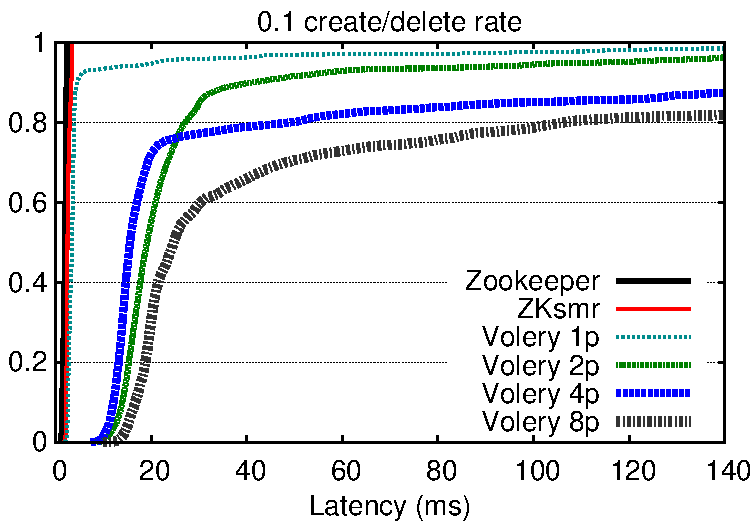
\includegraphics[width=0.9\columnwidth]{{graphs/results/zk_multipartition/plot_latency_cdfs_globalrate_0.1}.pdf}
\end{minipage}
\caption{Cumulative distribution function (CDF) of latency for different rates of create/delete commands (in-memory storage, 1000-bytes commands).}
\label{fig:zkglobalcdf}
\end{figure*}



We can see in Figure \ref{fig:zkglobal} (top left) that Volery scales throughput with the number of partitions for all configurations but the exceptional case of 10\% of global commands when augmenting the number of partitions from 4 to 8.
Moreover, Volery with two partitions outperforms the Zookeeper in all experiments.
The major drawback of Volery under global commands is that to ensure linearizability, partitions must exchange signals: as \verb#create# and \verb#delete# commands are multicast to all partitions, no server can send a reply to a client before receiving a signal from \emph{all} other partitions when executing such a command. 
This explains the significant increase in latency shown in Figure \ref{fig:zkglobal} (bottom left), as global commands are added to the workload: as the number of partitions increases, so does the average latency. 
As we can see in Figure \ref{fig:zkglobal} (right), this extra latency comes from the servers waiting for signals from other partitions.

Figure \ref{fig:zkglobalcdf} shows the latency CDFs for the workloads with global commands. 
For experiments with more than one partition, the rate of messages with high latency is much higher than the rate of global commands. 
This happens due to a ``convoy effect": local commands may be delivered after global commands, having to wait for the latter to finish.
%This happens due to a ``convoy effect": local commands may be delivered after global commands and, therefore, must wait for the latter to finish executing.%, which delays the execution of the local commands.

%\subsection{Chirper experiments}
%
%TODO: every request touching x partitions; 1 experiment for each x in \{1, 2, 4, 8\}, when the system has p partitions, with p in \{1, 2, 4, 8\}
%
%We have also simulated a social network using detailed statistics of real Twitter usage, which can be found online.\footnote{http://www.sysomos.com/insidetwitter/} In such experiment, we simulated 100,000 users. Each user followed $f$ friends, where such friends were divided among $p$ partitions. The resulting graph was made so that each user would have $r$ followers. For each user, we decide values $f$, $p$ and $r$ randomly, based on the statistics we have found: we made both $f$ and $r$ follow a Zipfian distribution with size 100 and skew 1, while $p$ followed a Zipfian distribution with size $P$ (total number of partitions in the system) and skew 1. Also, according to the statistics we have used, 5\% of all Twitter users were responsible for 75\% of all Twitter activity (i.e., number of tweets), while 10\% were responsible for 86\% of all activity, and so on, approximately fitting a Zipfian distribution with size 100 and skew 1.6, where the most active users were the ones with most followers, so our simulated social network also had this characteristic. We used the same distribution for timeline requests, having the users with most friends (i.e., those who follow the most people) requesting their timeline more frequently than other users.

\section{Related work}
\label{sec:rw}

State machine replication~\cite{Lam78, Sch90, Kapritsos:2012um, kotla2004htbft, santos2013htsmr} is known for its strong consistency guarantees, which comes from the assumption of deterministic execution.
Its drawback is that such a determinism is usually ensured by having every replica executing the same commands, in the same order---that is, sequentially.
Since consistent ordering is fundamental for SMR, some authors proposed to optimize the ordering and propagation of commands (i.e., the atomic broadcast layer of the system).
For instance, \cite{kapritsos2010scalable} proposes to divide the ordering of commands between different clusters: each cluster orders only some requests, and then forwards the partial order to every server replica, which then merges the partial orders deterministically into a single total order that is consistent across the system.
In~\cite{biely2012spaxos}, Paxos~\cite{Lamport:1998ea} is used to order commands, but it is implemented in a way that avoids overloading the leader process, which would turn it into a bottleneck.

Multi-threaded execution is a potential source of non-determinism, depending on how threads are scheduled to be executed in the operating system.
Some works attempted to circumvent this problems and come up with a multi-threaded, yet deterministic implementation of SMR.
In \cite{santos2013htsmr}, the authors propose to parallelize the receival and dispatching of commands, while still executing commands sequentially.
In \cite{kotla2004htbft}, application semantics is used to determine which commands can be executed concurrently and still produce a deterministic outcome (e.g., read-only commands).
In \cite{Kapritsos:2012um}, commands are tentatively executed in parallel.
After the parallel execution, replicas verify whether they reached a consistent state; if not, commands are rolled back and re-executed sequentially.

Many database replication schemes aim at achieving higher throughput by relaxing consistency, that is, they do not ensure linearizability.
In deferred-update replication \cite{sciascia2012sdur, chundi96dur, kobus2013hybrid, SousaOMP01}, replicas commit read-only transactions immediately, not always synchronizing with each other.
Although this indeed improves performance significantly, it allows non-linearizable executions to take place; database systems usually ensure serializability \cite{BHG87} or snapshot isolation \cite{LinKJPA09}.
Those criteria can be considered weaker than linearizability, in the sense that they do not take into account real-time precedence of different commands among different clients. 
For some applications, these consistency levels may be enough, allowing the system to scale better, but services that require linearizability cannot be implemented with such techniques.

Efforts to make linearizable systems scalable have been made in the past~\cite{corbett2013spanner, bezerra2014ssmr, le2016dssmr, Glendenning2011, Marandi11}.
In \cite{Glendenning2011}, the authors propose a scalable key-value store based on DHTs, ensuring linearizability, but only for requests that access the same key. 
In \cite{Marandi11}, a partitioned variant of SMR is proposed.
However, it requires total order (i.e., all commands have to be ordered against each other) and it does not allow a single command to update variables in different partitions.
Spanner~\cite{corbett2013spanner} uses a separate Paxos group per partition and, to ensure strong consistency across partitions, clocks are assumed to be synchronized.
Although the authors say that Spanner works well with GPS and atomic clocks, if clocks go out of synch beyond the tolerated difference, correcteness is not guaranteed.
\ssmr{}~\cite{bezerra2014ssmr} ensures consistency across partitions without any assumption about clock synchronization, but relying on a static partitioning of the state.
\dssmr{}~\cite{le2016dssmr} extends S-SMR by allowing state variables to migrate across partition in order to reduce multi-partition commands.
However, \dssmr{} implements repartitioning in a very simple way that does not perform very well in scenarios with weak locality.
\dynastar\ improves on DS-SMR by employing well known graph partitioning techniques to decide where each variable should be.
Moreover, \dynastar\ dillutes the cost of repartitioning by moving variables on-demand, that is, only when they are accessed by some command.

\eb{I'm not sure if this paragraph should stay here; I'd vote to remove it...}
\dynastar\ is not to be confused with other dynamic replication schemes though.
Systems such as~\cite{birman2010dsr,guessoum2003dar,dustdar2007soc} are ``dynamic'' in the sense that they allow the membership to be reconfigured during execution.
For instance, a multicast layer based on Paxos can be reconfigured by adding or removing acceptors. They also allow server replicas to be added and removed during execution.
However, this is orthogonal to what \dynastar\ proposes.
\dynastar\ consists of allowing the \emph{state partitioning}, that is, which state variables belong to which partition, to change dynamically.
The greatest challenge that is addressed by \dynastar\ is how to provide such a solution, with a dynamic partitioning oracle, while ensuring a very strong level of consistency (linearizability), as variables are created, deleted, and moved across partitions, based on the access patterns of the workload.

Graph-partitioning is an interesting problem with many proposed solutions~\cite{Abou-Rjeili:2006,kernighan1970efficient,hendrickson2000graph}.
In this work, we do not introduce a new graph partitioning solution, but instead we use a well-known one (Metis~\cite{Abou-Rjeili:2006}) to partition the state of a service implemented with state machine replication.
Similarly to \dynastar{}, Schism~\cite{curino2010sch} also uses graph-based partitioning to decide where to place data items in a transactional database.
The authors propose to use the workload to create a graph that captures dependencies between data items, but not much detail is given about how the repartitioning can be done dynamically without violating consistency.
Sword~\cite{quamar2013sword} is another graph-based dynamic repartitioning technique.
It uses a hypergraph partitioning algorithm do distributes rows of tables in a relational database across database shards.
However, it does address linearizability.
E-Store~\cite{taft2014est} is yet another repartitioning proposal for transactional databases.
It repartitions data according to access patterns from the workload.
It strives to minimize the number of multi-partition accesses and is able to redistribute data items among partitions during execution.
However, E-Store assumes that all non-replicated tables form a tree-schema based on foreign key relationships.
This has the drawback of ruling out graph-structured schemas and \mbox{$m$-$n$} relationships.
\dynastar\ is a more general approach that works with any kind of relationship between data items, while also ensuring linearizability.

\section{Conclusion}


\section*{Acknowledgements}
\label{sec:acknowledgements}

This work was supported in part by the Swiss National Science Foundation under grant number 146404. Robbert van Renesse is supported in part by grants from AFOSR, NSF, DARPA, ARPA-e, MDCN/iAd, Microsoft Corporation, Facebook Inc., and Amazon.com.% We also thank Samuel Benz and Leandro Pacheco de Sousa for the discussions.

%\section*{Acknowledgment}
%Thank the reviewrs

%\bibliographystyle{IEEEtran}
\bibliographystyle{ieeetr}
%\bibliographystyle{abbrvnat}
\bibliography{references_short}
%\bibliography{references}



\end{document}